% Aegis-v2 research paper (IEEE two-column journal format).
% Build: see researchpaper/README.md  (pdflatex -> bibtex -> pdflatex -> pdflatex)
% Tables in tables/*.tex and figures in figures/*.pdf are generated from the result files by
% make_paper_tables.py and make_paper_figures.py; do not edit them by hand.
\documentclass[journal]{IEEEtran}

\usepackage[T1]{fontenc}
\usepackage{amsmath,amssymb}
\usepackage{graphicx}
\usepackage{booktabs}
\usepackage{array}
\usepackage{cite}
\usepackage{url}
\usepackage{xcolor}
\usepackage{tikz}
\usetikzlibrary{arrows.meta,positioning,fit,calc,shapes.geometric,backgrounds,decorations.pathreplacing,decorations.pathmorphing}
\usepackage{algorithm}
\usepackage{algorithmic}
\usepackage[hidelinks]{hyperref}

\definecolor{aegis}{HTML}{2A78D6}
\definecolor{scrub}{HTML}{EB6834}
\definecolor{crit}{HTML}{D93A3A}
\definecolor{good}{HTML}{128A5A}
\definecolor{warnc}{HTML}{B97A00}
\definecolor{flash}{HTML}{F2B33D}
\definecolor{uplinkc}{HTML}{008300}
\definecolor{rangerc}{HTML}{1BAF7A}

\newcommand{\aegis}{Aegis-v2}
\newcommand{\pmci}[1]{{\scriptsize$\pm$#1}}
\renewcommand{\algorithmicrequire}{\textbf{Input:}}
\renewcommand{\algorithmicensure}{\textbf{Output:}}

\hyphenation{Res-Net Euro-SAT}

% Generated table bodies are read with the primitive \input, which is expandable inside tabular
\makeatletter\newcommand{\tablebody}[1]{\@@input #1 }\makeatother

\begin{document}

\title{Aegis-v2: Detection-Gated, Layer-Selective\\ Self-Repair of Onboard Earth-Observation\\ Classifiers under Orbit-Calibrated Radiation Upsets}

\author{RG~Saran~Vishakan%
\thanks{R.\,G.~Saran~Vishakan is with [Department, Institution] (e-mail: rgsaranvishakan2006@gmail.com).}%
\thanks{Code, campaign results, the analysis scripts that generate every table and figure, and an interactive mission dossier are available in the project repository (\texttt{Rg9906/aegis-v2}).}}

\markboth{Preprint, October 2026}{Saran Vishakan: Aegis-v2, Detection-Gated Self-Repair of Onboard Classifiers}

\maketitle

\begin{abstract}
Deep neural networks now run on commercial off-the-shelf (COTS) processors aboard Earth-observation satellites,
where single-event upsets (SEUs) from trapped protons silently corrupt the stored weights. In IEEE-754 single
precision, one flip of the most significant exponent bit turns a weight of order one into a value near $10^{38}$ and
collapses a classifier to chance. Existing remedies sit at two extremes: blind periodic scrubbing rewrites the whole
model on a timer, while in-situ software mitigation (activation clipping, batch-norm re-centering) leaves corrupted
weights in memory, where they accumulate. We present \aegis{}, a detection-gated, layer-selective repair loop. A
label-free behavioral monitor (an activation-range envelope and a batch-norm drift test) proposes suspect blocks on
each incoming image batch; a CRC-32 comparison against golden checksums confirms which blocks actually changed,
including the block just upstream of the earliest alarm; only confirmed blocks are restored, bit-exactly, from a
compressed golden copy in radiation-tolerant storage. An optional periodic CRC audit catches faults too small to change
behavior. We evaluate \aegis{} in a paired, seeded mission simulator that flies a real Sentinel-2A track (SGP4),
defines the South Atlantic Anomaly physically from IGRF field strength, and calibrates upset rates to eight years of
Alsat-1 flight data. Over three simulated days and three radiation seeds on EuroSAT, \aegis{} keeps a ResNet-18 at
$87.4\%$ mean accuracy (clean $89.3\%$) and within five points of clean for $89\%$ of the mission, against $37.0\%$ and
$26\%$ for 12-hour scrubbing, $38.5\%$ for range clipping and $14.0\%$ unprotected, winning every paired seed; matching
its accuracy by scrubbing would take $4.7\times$ the repair traffic. A held-out-trained MobileNetV2 keeps clean accuracy
at $3.4$\,MB/day. An exact ablation on identical fault streams shows that the upstream-block rule prevents a 35-hour
outage. In 300 controlled single upsets, only exponent-MSB flips caused damage, and every damaging flip was detected and localized with no false restore; damaged classifiers collapse toward a single, fault-dependent land-cover class. We
also report a negative result: always-on monitoring makes \aegis{} cost $5$--$22\times$ more energy than slow scrubbing
under our energy model, so its advantage is bandwidth and availability, not energy. We document the evaluation
pitfalls that invalidated our own early results and release the simulator, campaigns and analysis scripts.
\end{abstract}

\begin{IEEEkeywords}
Single-event upset, soft errors, fault tolerance, onboard machine learning, Earth observation, deep neural networks,
self-repair, South Atlantic Anomaly, memory scrubbing, batch normalization.
\end{IEEEkeywords}

% =====================================================================================================
\section{Introduction}
\IEEEPARstart{O}{nboard} inference has moved from demonstration to routine. $\Phi$-Sat-1 flew a convolutional cloud
screener on a COTS vision accelerator in 2020 and discarded cloudy frames before downlink~\cite{giuffrida2022phisat};
OPS-SAT trained and replaced models in orbit~\cite{opssat}; current small-satellite payloads carry Jetson-class GPUs
and neural accelerators~\cite{furano2020edge,rednet2024}; and system papers now treat AI services in orbit as
infrastructure~\cite{aispace2026}. The appeal is plain: the downlink is the bottleneck of Earth observation, so deciding
onboard what is worth sending multiplies the useful data a satellite returns. The cost is reliability. COTS processors
and memories are not radiation hardened, and in low Earth orbit (LEO) energetic protons trapped in the inner Van Allen
belt, concentrated over the South Atlantic Anomaly (SAA)~\cite{heirtzler2002saa}, deposit enough charge to flip stored
bits~\cite{baumann2005soft,petersen2011see}.

A neural network is an unusually fragile thing to store in such memory. Its knowledge lives in millions of
floating-point weights, and the IEEE-754 binary32 format~\cite{ieee754} packs an 8-bit exponent beside the sign.
Trained weights are small, so their exponent's most significant bit is almost always zero; flipping it multiplies the
weight by $2^{128}\approx3.4\times10^{38}$. One such upset in a convolution kernel saturates every activation
downstream and drives the classifier to chance, as targeted bit-flip attacks showed on purpose~\cite{rakin2019bfa} and
statistical injection studies confirm for vision transformers~\cite{sentry2026}. Upsets also accumulate: unlike a
transient glitch in logic, a flipped bit in SRAM or DRAM stays flipped until something rewrites it.

Spacecraft engineering answers with hardware: error-detecting and correcting codes (EDAC), triple modular redundancy
and memory scrubbing, the periodic rewriting of memory from a trusted copy~\cite{petersen2011see,bentoutou2011edac,noldeke2021flp}.
Scrubbing is simple and robust but blind: it pays to rewrite the whole model whether or not anything is wrong, and
between scrubs the model runs corrupted. The machine-learning community answers with software. Range restriction
(Ranger~\cite{chen2021ranger}, FT-ClipAct~\cite{hoang2020ftclipact}) clamps activations to profiled bounds;
BLINK~\cite{blink2026} detects batch-norm drift and re-centers activations; RADAR~\cite{li2021radar} and
MILR~\cite{ponader2021milr} detect or algebraically recover corrupted weights; fault-aware training hardens the weights
themselves~\cite{vinck2025fat}. These methods mitigate symptoms in place but, with the exception of algebraic recovery,
leave the corrupted weights in memory, where further upsets compound them. A third option is to wait for a ground
station and re-upload the model, which costs scarce uplink time and leaves the model broken until the next contact.
Fig.~\ref{fig:concept} contrasts the four behaviors on one fault sequence.

\begin{figure}[t]
\centering
\resizebox{\columnwidth}{!}{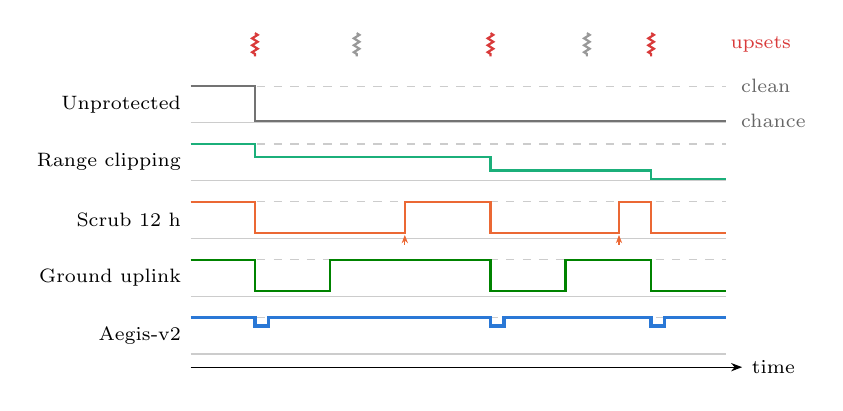
\begin{tikzpicture}[x=0.68cm,y=0.42cm,font=\scriptsize]
  % time axis and fault marks
  \foreach \t/\c in {1.2/crit,3.1/black!40,5.6/crit,7.4/black!40,8.6/crit} {
    \draw[\c,thick,decorate,decoration={zigzag,segment length=2.5pt,amplitude=1pt}] (\t,9.6) -- (\t,8.9);
  }
  \node[anchor=west,crit] at (9.9,9.25) {upsets};
  \foreach \row/\name/\col in {0/{Unprotected}/black!55,1/{Range clipping}/rangerc,2/{Scrub 12 h}/scrub,3/{Ground uplink}/uplinkc,4/{\aegis{}}/aegis} {
    \pgfmathsetmacro{\yb}{6.9-1.75*\row}
    \node[anchor=east] at (0,\yb+0.55) {\name};
    \draw[black!20] (0,\yb) -- (10,\yb);
    \draw[black!20,dashed] (0,\yb+1.1) -- (10,\yb+1.1);
  }
  % unprotected: falls at 1.2 and stays
  \draw[black!55,thick] (0,8.0) -- (1.2,8.0) -- (1.2,6.95) -- (10,6.95);
  % clipping: partial drops that accumulate
  \draw[rangerc,thick] (0,6.25) -- (1.2,6.25) -- (1.2,5.85) -- (5.6,5.85) -- (5.6,5.45) -- (8.6,5.45) -- (8.6,5.2) -- (10,5.2);
  % scrub: falls, recovers at 4 and 8
  \draw[scrub,thick] (0,4.5) -- (1.2,4.5) -- (1.2,3.55) -- (4,3.55) -- (4,4.5) -- (5.6,4.5) -- (5.6,3.55) -- (8,3.55) -- (8,4.5) -- (8.6,4.5) -- (8.6,3.55) -- (10,3.55);
  \foreach \x in {4,8} \draw[scrub,-{Stealth[length=3pt]}] (\x,3.2) -- (\x,3.5);
  % uplink: recovers only at contacts 2.6 and 7
  \draw[uplinkc,thick] (0,2.75) -- (1.2,2.75) -- (1.2,1.8) -- (2.6,1.8) -- (2.6,2.75) -- (5.6,2.75) -- (5.6,1.8) -- (7,1.8) -- (7,2.75) -- (8.6,2.75) -- (8.6,1.8) -- (10,1.8);
  % aegis: dips one step at each critical upset, then restored
  \draw[aegis,very thick] (0,1.0) -- (1.2,1.0) -- (1.2,0.75) -- (1.45,0.75) -- (1.45,1.0) -- (5.6,1.0) -- (5.6,0.75) -- (5.85,0.75) -- (5.85,1.0) -- (8.6,1.0) -- (8.6,0.75) -- (8.85,0.75) -- (8.85,1.0) -- (10,1.0);
  \draw[-{Stealth[length=4pt]}] (0,-0.5) -- (10.3,-0.5) node[right] {time};
  \node[anchor=west,black!60] at (10.1,8.0) {clean};
  \node[anchor=west,black!60] at (10.1,6.95) {chance};
\end{tikzpicture}}
\caption{Schematic behavior of the strategies on one sequence of upsets (red: damaging; grey: harmless). Clipping
softens each hit but cannot undo it; scrubbing recovers only on its timer; a ground reload only at contacts; \aegis{}
detects and restores the damaged block at the next monitored batch and ignores harmless hits.}
\label{fig:concept}
\end{figure}

This paper asks whether a satellite can do better by combining the two worlds: use cheap, label-free signals from the
network's own activity to notice damage, use exact checksums to prove which stored blocks changed, and then restore
only those blocks from an onboard golden copy. We call this \emph{detection-gated, layer-selective restore} and build
it as \aegis{}. The idea is simple; demonstrating it honestly is not. Evaluations of DNN resilience are easy to get
wrong in ways that flatter the method: unrealistic fault models (zeroed weights instead of exponent
flips)~\cite{dossantos2023neutron}, synthetic inputs, monitors whose thresholds fire on every clean batch, energy
budgets that omit the monitor itself. Our own first prototype reported a $98.9\%$ energy saving that did not survive
correction (Section~\ref{sec:lessons}). We therefore treat the evaluation methodology as a first-class contribution.

\textbf{Contributions.}
\begin{enumerate}
  \item \textbf{A detection-gated, layer-selective repair loop} (\aegis{}) that combines a two-tier label-free
  behavioral monitor with CRC-32 confirmation, an \emph{upstream-block rule} that localizes batch-norm parameter
  faults whose symptoms appear one block downstream, and an optional periodic CRC audit (Section~\ref{sec:method}).
  \item \textbf{A paired, orbit-calibrated mission simulator}: faults placed uniformly over stored bits at rates
  integrated minute by minute along a real Sentinel-2A track, with the SAA defined from IGRF field strength and the
  orbit-mean rate calibrated to Alsat-1 flight data; every strategy replays the identical fault stream
  (Section~\ref{sec:faultmodel}).
  \item \textbf{A head-to-head evaluation} on two architectures against no protection, range clipping, BN
  re-centering, periodic scrubbing at five intervals and a ground-uplink reload, reporting mean accuracy, availability,
  accuracy-loss area, repair traffic and modeled energy with 95\% intervals and paired differences
  (Section~\ref{sec:results}).
  \item \textbf{An exact ablation and a single-fault detection study}: the upstream rule is isolated on identical
  fault streams, and 300 controlled single upsets measure what each tier detects, by bit field, and what a damaged
  classifier predicts (Sections~\ref{sec:ablation}--\ref{sec:collapse}).
  \item \textbf{An honest cost accounting with a negative result}: with monitor compute charged, \aegis{} is not an
  energy saver (Section~\ref{sec:costs}).
  \item \textbf{A catalogue of evaluation pitfalls}, each of which silently invalidated a result during this work, with
  the invariant that prevents it (Section~\ref{sec:lessons}).
\end{enumerate}

% =====================================================================================================
\section{Background}
\label{sec:background}

\subsection{Radiation in Low Earth Orbit}
In LEO the dominant source of SEUs in memory is the flux of trapped protons in the inner radiation belt, supplemented
by galactic cosmic rays and solar particle events~\cite{petersen2011see}. Because Earth's dipole is offset and tilted,
the inner belt reaches its lowest altitude over the South Atlantic, where the field strength at a given altitude is
weakest; this is the SAA~\cite{heirtzler2002saa}. A sun-synchronous satellite crosses it on several consecutive orbits
each day, and most memory upsets on such missions are recorded inside it. Flight missions handle this with EDAC and
background scrubbing of program memory; the Flying Laptop mission documents in-flight SEU statistics and scrubbing
operations~\cite{noldeke2021flp}.

The Alsat-1 record is unusually useful for calibration: between November 2002 and August 2010 its commercial SRAM
logged 265,649 upsets in 2,622 days, i.e.\ $4.04\times10^{-7}$ upsets/bit/day, of which $98.55\%$ were single-bit upsets
(SBUs) and the remainder multiple-bit upsets (MBUs); the yearly mean rose from 41 to 119 upsets per day over the solar
cycle~\cite{bentoutou2011edac}.

\subsection{Why Floating-Point Weights Are Fragile}
\begin{figure}[t]
\centering
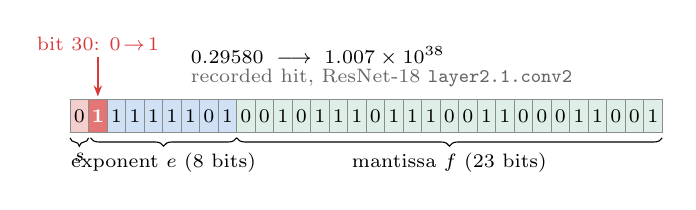
\begin{tikzpicture}[x=0.235cm,y=0.42cm,font=\scriptsize]
  \foreach \i in {0,...,31} {
    \pgfmathtruncatemacro{\b}{31-\i}
    \ifnum\b=31 \def\fc{crit!25}\else\ifnum\b>22 \def\fc{aegis!22}\else\def\fc{good!14}\fi\fi
    \ifnum\b=30 \def\fc{crit!70}\fi
    \filldraw[fill=\fc,draw=black!45,line width=0.3pt] (\i,0) rectangle ++(1,1);
  }
  \node at (0.5,0.5) {0};
  \node[text=white,font=\scriptsize\bfseries] at (1.5,0.5) {1};
  \foreach \i/\v in {2/1,3/1,4/1,5/1,6/1,7/0,8/1,9/0,10/0,11/1,12/0,13/1,14/1,15/1,16/0,17/1,18/1,19/1,20/0,21/0,22/1,23/1,24/0,25/0,26/0,27/1,28/1,29/0,30/0,31/1}
    \node at (\i+0.5,0.5) {\v};
  \draw[decorate,decoration={brace,amplitude=3pt,mirror}] (0,-0.15) -- (1,-0.15) node[midway,below=2pt] {$s$};
  \draw[decorate,decoration={brace,amplitude=3pt,mirror}] (1.1,-0.15) -- (9,-0.15) node[midway,below=2pt] {exponent $e$ (8 bits)};
  \draw[decorate,decoration={brace,amplitude=3pt,mirror}] (9,-0.15) -- (32,-0.15) node[midway,below=2pt] {mantissa $f$ (23 bits)};
  \draw[-{Stealth[length=4pt]},crit,thick] (1.5,2.3) -- (1.5,1.1);
  \node[crit,anchor=south,align=center] at (1.5,2.2) {bit 30: $0\!\to\!1$};
  \node[anchor=west,align=left] at (6,2.0) {$0.29580 \;\longrightarrow\; 1.007\times10^{38}$\\[-1pt]\textcolor{black!60}{recorded hit, ResNet-18 \texttt{layer2.1.conv2}}};
\end{tikzpicture}
\caption{IEEE-754 binary32 layout of a weight hit during our campaign (ResNet-18, seed~1, hour~2). Flipping the most
significant exponent bit multiplies the value by $2^{128}$. Mantissa flips, $72.5\%$ of all recorded hits, change the
value by at most a factor of two.}
\label{fig:float}
\end{figure}

A binary32 value is $v=(-1)^{s}\,2^{e-127}\,(1+f)$ with sign $s$, biased exponent $e\in[1,254]$ for normal numbers, and
fraction $f\in[0,1)$ (Fig.~\ref{fig:float}). Table~\ref{tab:bitfields} summarizes what one flip does. A flip in mantissa
bit $k$ changes $1+f$ by $\pm2^{k-23}$, a factor between $2/3$ and $3/2$ at worst, so most mantissa flips are invisible
to a classifier. A flip in exponent bit $j\in[23,30]$ multiplies $v$ by $2^{\pm 2^{j-23}}$. Trained weights satisfy
$|v|<2$, so $e\le127$ and bit 30 is zero; a flip sets it and multiplies the value by exactly $2^{128}$, producing either a
huge finite value or $\pm\infty$. A sign flip on a batch-norm running variance makes $\sqrt{\sigma^2+\epsilon}$ undefined
and yields NaN. Under uniform placement about one hit in 32 lands on bit 30; we recorded $4.89$ such hits per day on
ResNet-18 against $4.6$ expected.

\begin{table}[t]
\centering
\caption{Effect of a single flip by bit field in a trained binary32 weight ($|v|<2$).}
\label{tab:bitfields}
\setlength{\tabcolsep}{3pt}
\begin{tabular}{@{}lccl@{}}
\toprule
Field (bits) & Share & Multiplier on $|v|$ & Typical consequence \\
\midrule
Sign (31) & $1/32$ & $1$ (sign change) & NaN if on a BN variance \\
Exponent MSB (30) & $1/32$ & $2^{128}$ & activation explosion \\
Exponent (23--29) & $7/32$ & $2^{\pm1}\ldots2^{\pm64}$ & small to catastrophic \\
Mantissa (0--22) & $23/32$ & $[2/3,\,3/2]$ & usually negligible \\
\bottomrule
\end{tabular}
\end{table}

\subsection{Onboard Earth-Observation Classification}
We use land-use/land-cover classification of Sentinel-2~\cite{drusch2012sentinel2} imagery as the workload, with the
EuroSAT benchmark~\cite{helber2019eurosat}: 27,000 RGB chips of $64\times64$ pixels in ten classes (Annual Crop, Forest,
Herbaceous Vegetation, Highway, Industrial, Pasture, Permanent Crop, Residential, River, Sea/Lake). The models are a
ResNet-18~\cite{he2016resnet} and a MobileNetV2~\cite{sandler2018mobilenetv2}, both with batch
normalization~\cite{ioffe2015bn}, the two families most often proposed for onboard vision.

% =====================================================================================================
\section{Related Work}
\label{sec:related}

\textbf{Hardware mitigation.} EDAC/ECC, selective or full TMR, and scrubbing remain the default for flight software
memory~\cite{petersen2011see,bentoutou2011edac,noldeke2021flp}. ECC adapted to DNN weights corrects single-bit errors and
masks uncorrectable weights, at $47.5\%$ area overhead~\cite{eccdnn2025}; Safe-NEureka adds dual-modular redundancy with
hardware recovery to a satellite DNN accelerator, protecting memory with ECC and the controller with
TMR~\cite{safeneureka2026}; ZEDAC protects model parameters in memory and storage with row/column extended-Hamming codes
held in a rad-tolerant companion, restoring corrupted parameters without retraining when errors stay within its
correctable regime~\cite{zedac2026}. Beam experiments caution that up to $61\%$ of DNN errors on GPUs were critical,
that ECC did little to reduce them, and that single-bit injection underestimated the measured misdetection rate of
YOLOv3 by $8.66\times$~\cite{dossantos2023neutron}. \aegis{} is complementary: it assumes a protected golden copy and
repairs the unprotected working copy.

\textbf{Algorithm-based fault tolerance and checksums.} ABFT~\cite{huang1984abft} and its convolutional descendants
detect computation errors via checksums; RADAR~\cite{li2021radar} compares group checksums of weights against golden
signatures and zeroes flagged groups; weight reconstruction~\cite{li2020reconstruction} defends against targeted
bit-flip attacks, which, like radiation, are most damaging in the exponent MSB~\cite{rakin2019bfa}. We use the simplest
member of this family, CRC-32~\cite{peterson1961crc} per block, but only as a confirmer gated by behavior.

\textbf{Range restriction.} Ranger~\cite{chen2021ranger}, FT-ClipAct~\cite{hoang2020ftclipact} and
ProAct~\cite{proact2024} clamp activations to bounds profiled on clean data; Ranger reports $3$--$50\times$ resilience
gains for transient faults at negligible cost. They need no storage, but they do not repair weights; under accumulating
upsets the clipped network degrades, which our ResNet-18 results confirm. RedNet combines such tolerance with
application awareness and early exit, and was validated on the Chaohu-1 SAR satellite payload~\cite{rednet2024}.

\textbf{Batch-norm based detection.} BLINK~\cite{blink2026} uses batch-norm statistics as integrity checkpoints,
reporting over $99\%$ detection precision and recovering ResNet-50/CIFAR-10 from $10\%$ to $85.9\%$ under $0.5\%$ random
bit flips with under $2\%$ latency overhead. Our Tier~2 is BLINK-style, and our BLINK baseline implements its
re-centering mitigation. The difference is what happens next: \aegis{} restores weights instead of compensating for them.

\textbf{Weight correction, hardening and analysis.} MILR~\cite{ponader2021milr} recovers layers algebraically from
stored input/output relations; CoG-guided correction~\cite{cog2026} substitutes profiled values for detected faulty
weights, reporting up to $49.6\times$ fault-tolerance improvement on ResNet-18; fault-aware training improves tolerance
to multiple SEUs by up to $3\times$~\cite{vinck2025fat}. Layer- and bit-wise sensitivity analyses exist for semantic
segmentation~\cite{gutierrez2024segmentation} and for vision transformers on EuroSAT, where only about $3\%$ of FP32
flips cause failure but most failures are severe and concentrate in normalization layers and exponent
bits~\cite{sentry2026}. Plasticity methods such as ReDo~\cite{sokar2023redo} and continual
backpropagation~\cite{dohare2024plasticity} reinitialize dormant units during training; they cannot restore a specific
learned function after hardware faults.

\textbf{Space ML robustness and tooling.} Lange et al.\ surveyed the robustness of onboard ML to radiation, found that
not all faults are as damaging as prior work claimed, and reported that existing injection tools were hard to apply to
satellite models~\cite{lange2024mlspace}. Fault injectors such as PyTorchFI~\cite{mahmoud2020pytorchfi} and
Ares~\cite{reagen2018ares} established application-level injection as a valid proxy.

\begin{table}[t]
\centering
\caption{Capability comparison. (a)~label-free behavioral monitor; (b)~restores corrupted weights; (c)~no labels or
ground contact needed for recovery; (d)~evaluated under orbit-calibrated accumulating faults.}
\label{tab:related}
\setlength{\tabcolsep}{3.5pt}
\begin{tabular}{@{}lcccc@{}}
\toprule
Approach & (a) & (b) & (c) & (d) \\
\midrule
Periodic scrubbing~\cite{petersen2011see} & -- & blind & \checkmark & -- \\
ECC / ZEDAC~\cite{eccdnn2025,zedac2026} & -- & on read & \checkmark & -- \\
Ranger / FT-ClipAct~\cite{chen2021ranger,hoang2020ftclipact} & bounds & -- & \checkmark & -- \\
BLINK~\cite{blink2026} & BN & -- & \checkmark & -- \\
RADAR~\cite{li2021radar} & -- & zeroes group & \checkmark & -- \\
MILR~\cite{ponader2021milr} & -- & algebraic & \checkmark & -- \\
CoG correction~\cite{cog2026} & -- & substitutes & \checkmark & -- \\
RedNet~\cite{rednet2024} & -- & -- & \checkmark & flight \\
Ground re-upload & -- & late & -- & -- \\
\midrule
\textbf{\aegis{} (ours)} & \textbf{bounds+BN} & \textbf{CRC-gated} & \checkmark & \checkmark \\
\bottomrule
\end{tabular}
\end{table}

Table~\ref{tab:related} summarizes the gap. Every component of \aegis{} exists in isolation; to our knowledge the
combination, evaluated as a repair \emph{policy} under accumulating, orbit-modulated faults with paired baselines and
traffic and energy accounting, has not been reported.

% =====================================================================================================
\section{Fault Model and Mission Simulator}
\label{sec:faultmodel}

\subsection{What Is Corrupted}
Let the model's stored state be $\theta\in\mathbb{F}_{32}^{N}$, all parameters and batch-norm buffers, occupying
$B=32N$ bits: $358.1$\,Mbit for ResNet-18 ($44.77$\,MB) and $72.7$\,Mbit for MobileNetV2 ($9.08$\,MB). We model SEUs in
the working copy of $\theta$ held in volatile memory. Faults persist until a repair overwrites them. We do not inject
into activations, control logic or the golden copy, which we assume resides in radiation-tolerant non-volatile memory
(MRAM or rad-hard SPI NOR); transient activation faults are studied separately (Section~\ref{sec:transient}).

\subsection{Upset Arrival Along a Real Orbit}
The satellite follows Sentinel-2A (NORAD 40697, $\approx786$\,km sun-synchronous) propagated with
SGP4~\cite{vallado2006sgp4} from a CelesTrak two-line element set~\cite{celestrak}, sampled every minute. At each
position $\mathbf r(t)$ we evaluate the geomagnetic field magnitude $|B(\mathbf r)|$ from IGRF-13~\cite{alken2021igrf} and
map it to a per-bit upset rate by a linear ramp:
\begin{equation}
\lambda(t)=\lambda_{\mathrm{bg}}+(\lambda_{\mathrm{SAA}}-\lambda_{\mathrm{bg}})\,
\mathrm{clip}\!\left(\frac{B_{\mathrm{e}}-|B(\mathbf r(t))|}{B_{\mathrm{e}}-B_{\mathrm{c}}},0,1\right),
\label{eq:rate}
\end{equation}
with edge $B_{\mathrm e}=20{,}000$\,nT and core $B_{\mathrm c}=18{,}000$\,nT. The number of upsets in a step of length
$\Delta$ is Poisson with mean $B\int_{t}^{t+\Delta}\lambda(\tau)\,d\tau$, integrated per minute. Fig.~\ref{fig:orbit}
shows one day of the track over the field and Fig.~\ref{fig:rate} the resulting rate: background most of the day,
punctuated by roughly ten short SAA passes, several of which reach the core rate.

\begin{figure}[t]
\centering
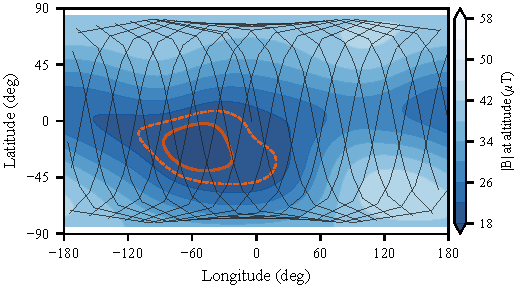
\includegraphics[width=\columnwidth]{figures/fig_orbit.pdf}
\caption{One day of the Sentinel-2A ground track (SGP4) over IGRF field magnitude at altitude. Solid and dashed
contours mark the SAA core ($18{,}000$\,nT) and edge ($20{,}000$\,nT) between which the upset rate ramps.}
\label{fig:orbit}
\end{figure}

\begin{figure*}[t]
\centering
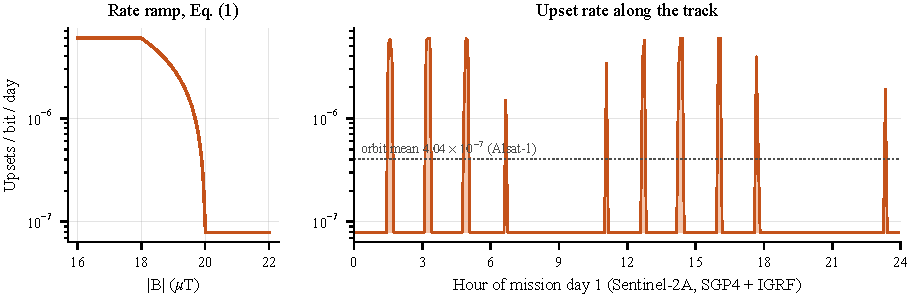
\includegraphics[width=\textwidth]{figures/fig_rate.pdf}
\caption{Left: the rate ramp of Eq.~(\ref{eq:rate}). Right: the per-bit upset rate along the first mission day. Upsets
arrive in short bursts during SAA passes over a low background; the dotted line is the orbit mean, calibrated to
Alsat-1.}
\label{fig:rate}
\end{figure*}

\textbf{Calibration.} We fix the ratio $\lambda_{\mathrm{SAA}}/\lambda_{\mathrm{bg}}=75.3$ and choose
$\lambda_{\mathrm{bg}}=7.89\times10^{-8}$ and $\lambda_{\mathrm{SAA}}=5.94\times10^{-6}$ upsets/bit/day so that the orbit
average over the real track ($79.9$ SAA-core-equivalent minutes per day) reproduces the Alsat-1 mean of
$4.04\times10^{-7}$~\cite{bentoutou2011edac}. About $82\%$ of upsets then occur inside the SAA. Table~\ref{tab:faults}
checks the calibration against the campaigns: the predicted $B\bar\lambda$ matches the recorded flip rate on both
architectures, and the recorded field distribution matches uniform placement.

\begin{table}[t]
\centering
\caption{Fault statistics of the final campaigns (three seeds, three days each). Severity uses the rule of
Section~\ref{sec:faults}.}
\label{tab:faults}
\setlength{\tabcolsep}{3pt}
\begin{tabular}{@{}lrr@{}}
\toprule
 & ResNet-18 & MobileNetV2 \\
\midrule
\tablebody{tables/tab_faults.tex}
\bottomrule
\end{tabular}
\end{table}

\subsection{Placement and Multiplicity}
Each upset event is an SBU with probability $0.9855$, otherwise an MBU cluster of up to four adjacent bits. Events are
placed uniformly over stored bits: a block is chosen with probability proportional to its bit count, then a tensor in
proportion to its size, an element and a bit. All 32 bit positions are eligible; restricting injection to the exponent
would inflate severity.

\subsection{Paired Replay}
\begin{figure}[t]
\centering
\resizebox{\columnwidth}{!}{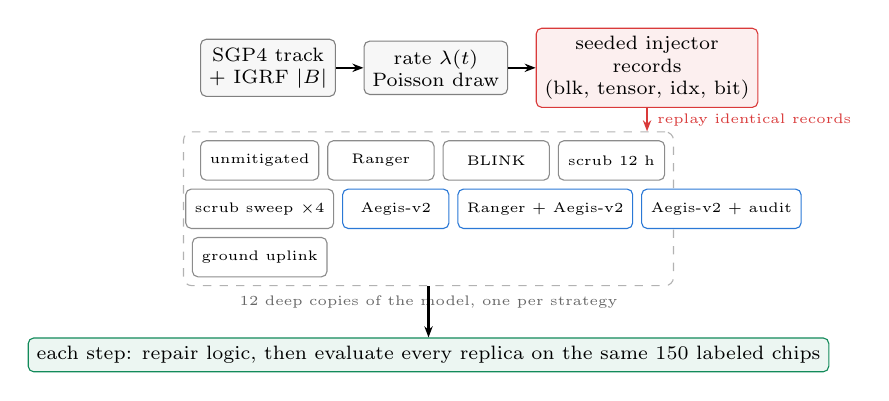
\begin{tikzpicture}[font=\scriptsize,
  box/.style={draw=black!50,rounded corners=2pt,align=center,inner sep=3pt,fill=black!3},
  rep/.style={draw=black!45,rounded corners=2pt,minimum width=1.35cm,minimum height=0.5cm,fill=white,font=\tiny},
  arr/.style={-{Stealth[length=4pt]},thick}]
  \node[box] (orb) {SGP4 track\\+ IGRF $|B|$};
  \node[box,right=0.35cm of orb] (rate) {rate $\lambda(t)$\\Poisson draw};
  \node[box,right=0.35cm of rate,fill=crit!8,draw=crit] (inj) {seeded injector\\records\\(blk, tensor, idx, bit)};
  \draw[arr] (orb) -- (rate);
  \draw[arr] (rate) -- (inj);
  \node[rep,below=0.55cm of orb.south west,anchor=north west] (r1) {unmitigated};
  \node[rep,right=0.1cm of r1] (r2) {Ranger};
  \node[rep,right=0.1cm of r2] (r3) {BLINK};
  \node[rep,right=0.1cm of r3] (r4) {scrub 12 h};
  \node[rep,below=0.1cm of r1] (r5) {scrub sweep $\times4$};
  \node[rep,right=0.1cm of r5,draw=aegis] (r6) {\aegis{}};
  \node[rep,right=0.1cm of r6,draw=aegis] (r7) {Ranger + \aegis{}};
  \node[rep,right=0.1cm of r7,draw=aegis] (r8) {\aegis{} + audit};
  \node[rep,below=0.1cm of r5] (r9) {ground uplink};
  \begin{scope}[on background layer]
    \node[draw=black!30,dashed,rounded corners=3pt,fit=(r1)(r4)(r9),inner sep=3pt,label={[font=\tiny,text=black!60]below:12 deep copies of the model, one per strategy}] (reps) {};
  \end{scope}
  \draw[arr,crit] (inj.south) -- node[right,font=\tiny,text=crit]{replay identical records} (inj.south |- reps.north);
  \node[box,below=0.65cm of reps,fill=good!8,draw=good] (eval) {each step: repair logic, then evaluate every replica on the same 150 labeled chips};
  \draw[arr] (reps) -- (eval);
\end{tikzpicture}}
\caption{Simulator data flow. One seeded injector samples each step's upsets; every replica replays the same records,
so the strategies differ only in how they respond and all comparisons within a seed are paired.}
\label{fig:sim}
\end{figure}

A single seeded injector samples the fault stream for the unprotected replica, recording
$(\text{block},\text{tensor},\text{index},\text{bit})$ tuples. Every other strategy runs on its own deep copy of the model
and \emph{replays the identical records} (Fig.~\ref{fig:sim}). Differences between strategies within a seed are
therefore paired, and we report paired differences with Student-$t$ intervals.

\subsection{Problem Statement}
A repair \emph{strategy} $\pi$ observes, at each step $t$, only the unlabeled incoming batch $X_t$ and its own model
state, and may rewrite any subset of blocks from the golden copy. Let $A_\pi(t)$ be the top-1 accuracy of its model on a
held-out labeled set after step $t$, $A_0$ the clean accuracy, $D_\pi(T)$ the bytes it moved and $E_\pi(T)$ the energy
it spent over a mission of $T$ steps of length $\Delta$. We evaluate
\begin{align}
\bar A_\pi&=\frac{1}{T}\sum_{t=1}^{T}A_\pi(t),\\
\mathcal U_\pi&=\frac{1}{T}\sum_{t=1}^{T}\mathbf{1}\!\left[A_\pi(t)\ge A_0-0.05\right],\\
\mathcal L_\pi&=\Delta\sum_{t=1}^{T}\max\!\left(A_0-A_\pi(t),0\right),
\end{align}
i.e.\ mean accuracy, availability (fraction of the mission within five points of clean) and accuracy-loss area in
point-hours, alongside $D_\pi$ and $E_\pi$, without labels or ground contact. No strategy need dominate on all
criteria; periodic scrubbing with interval $h$ traces a one-parameter family $\{(\bar A_h,D_h)\}$, the frontier any
detection-based policy must beat.

% =====================================================================================================
\section{The Aegis-v2 Method}
\label{sec:method}

\begin{figure*}[t]
\centering
\resizebox{\textwidth}{!}{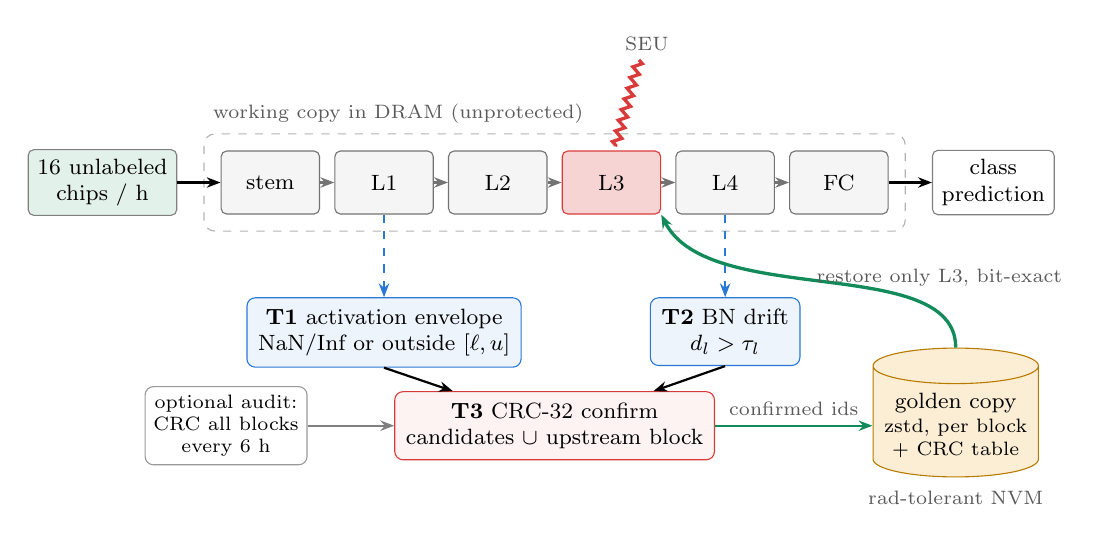
\begin{tikzpicture}[
  font=\footnotesize,
  blk/.style={draw=black!55,rounded corners=2pt,minimum width=1.25cm,minimum height=0.8cm,fill=black!4},
  hit/.style={blk,fill=crit!22,draw=crit},
  tier/.style={draw=aegis,rounded corners=3pt,fill=aegis!8,align=center,inner sep=4pt},
  store/.style={cylinder,shape border rotate=90,aspect=0.22,draw=warnc,fill=flash!22,minimum width=2.1cm,minimum height=1.25cm,align=center},
  arr/.style={-{Stealth[length=5pt]},thick},
  lab/.style={font=\scriptsize,text=black!65}
]
  \node[draw=black!50,fill=good!12,rounded corners=2pt,minimum width=1.3cm,minimum height=0.8cm,align=center] (in) at (0,0) {16 unlabeled\\chips / h};
  \node[blk,right=0.55cm of in] (b0) {stem};
  \node[blk,right=0.18cm of b0] (b1) {L1};
  \node[blk,right=0.18cm of b1] (b2) {L2};
  \node[hit,right=0.18cm of b2] (b3) {L3};
  \node[blk,right=0.18cm of b3] (b4) {L4};
  \node[blk,right=0.18cm of b4] (b5) {FC};
  \node[draw=black!50,rounded corners=2pt,minimum height=0.8cm,right=0.55cm of b5,align=center] (out) {class\\prediction};
  \draw[arr] (in) -- (b0);
  \foreach \a/\b in {b0/b1,b1/b2,b2/b3,b3/b4,b4/b5} \draw[arr,black!55] (\a) -- (\b);
  \draw[arr] (b5) -- (out);
  \begin{scope}[on background layer]
    \node[draw=black!30,dashed,rounded corners=4pt,fit=(b0)(b5),inner sep=6pt,label={[lab,anchor=south west]north west:working copy in DRAM (unprotected)}] (model) {};
  \end{scope}
  \draw[crit,very thick,decorate,decoration={zigzag,segment length=4pt,amplitude=1.5pt}] ($(b3.north)+(0.35,1.15)$) -- ($(b3.north)+(0.05,0.05)$);
  \node[crit,lab,anchor=south] at ($(b3.north)+(0.45,1.15)$) {SEU};
  \node[tier,below=1.05cm of b1] (t1) {\textbf{T1} activation envelope\\NaN/Inf or outside $[\ell,u]$};
  \node[tier,below=1.05cm of b4] (t2) {\textbf{T2} BN drift\\$d_l>\tau_l$};
  \node[tier,below=0.75cm of $(t1)!0.5!(t2)$,draw=crit,fill=crit!6] (t3) {\textbf{T3} CRC-32 confirm\\candidates $\cup$ upstream block};
  \draw[arr,aegis,dashed] (b1.south) -- (t1.north);
  \draw[arr,aegis,dashed] (b4.south) -- (t2.north);
  \draw[arr] (t1.south) -- (t3);
  \draw[arr] (t2.south) -- (t3);
  \node[store,right=2.0cm of t3] (gold) {golden copy\\[-1pt]\scriptsize zstd, per block\\[-1pt]\scriptsize + CRC table};
  \node[lab,below=0.05cm of gold,align=center] {rad-tolerant NVM};
  \draw[arr,good] (t3.east) -- node[above,lab]{confirmed ids} (gold.west);
  \draw[arr,good,very thick] (gold.north) .. controls +(0,1.2) and +(0.6,-1.2) .. node[right,lab,pos=0.55]{restore only L3, bit-exact} (b3.south east);
  \node[draw=black!40,rounded corners=3pt,align=center,inner sep=3pt,left=1.1cm of t3,font=\scriptsize] (aud) {optional audit:\\CRC all blocks\\every 6 h};
  \draw[arr,black!50] (aud) -- (t3);
\end{tikzpicture}}
\caption{\aegis{} repair loop. Hooks on each incoming batch feed the behavioral tiers T1 and T2, which propose
candidate blocks without labels. T3 recomputes CRC-32 over each candidate and the block upstream of the earliest
candidate, compares with golden checksums, and only blocks whose stored bits changed are restored from the compressed
golden copy. Cascade victims downstream of a corrupted block raise alarms but pass T3 and are left untouched.}
\label{fig:arch}
\end{figure*}

\aegis{} runs once per monitoring period (one hour in our experiments) on the batch of images the satellite has just
acquired. Fig.~\ref{fig:arch} gives the overview and Algorithm~\ref{alg:aegis} the procedure.

\subsection{Design Evolution: From Aegis-v1 to v2}
The design was shaped by what did not work (Table~\ref{tab:evolution}). A first prototype (Aegis-v1) borrowed from
plasticity research: it watched for ``dead'' low-firing neurons in a small multilayer perceptron, modeled faults as
zeroed weights, and revived neurons with noise or re-initialization in the spirit of ReDo~\cite{sokar2023redo} and
continual backpropagation~\cite{dohare2024plasticity}. A prior-art review showed three problems. The fault model was
wrong: SEUs in float32 weights create huge values, not dead units, so a dead-neuron monitor watches for the opposite
symptom. Re-initialization re-randomizes capacity but cannot recover a specific learned function without a training
signal, and an inference-only payload has neither gradients nor labels. And a flat MLP does not represent the
batch-normalized CNNs flown in practice. \aegis{} keeps the idea of a self-monitoring network but replaces each piece
with one grounded in the reliability literature.

\begin{table}[t]
\centering
\caption{From Aegis-v1 to \aegis{}: what changed and why.}
\label{tab:evolution}
\setlength{\tabcolsep}{3pt}
\begin{tabular}{@{}>{\raggedright\arraybackslash}p{1.5cm}>{\raggedright\arraybackslash}p{2.7cm}>{\raggedright\arraybackslash}p{3.45cm}@{}}
\toprule
Aspect & Aegis-v1 & \aegis{} (inspiration) \\
\midrule
Fault model & zeroed weights, dead neurons & uniform bit flips, Alsat-1 rates, real orbit~\cite{bentoutou2011edac} \\
Monitor & low-firing neuron counts & activation envelope (Ranger~\cite{chen2021ranger}) + BN drift (BLINK~\cite{blink2026}) \\
Confirmation & none & CRC-32 per block (RADAR-style~\cite{li2021radar}) \\
Repair & noise / re-init (ReDo~\cite{sokar2023redo}) & bit-exact restore from golden copy (scrubbing~\cite{petersen2011see}) \\
Model & MLP & ResNet-18, MobileNetV2 with BN \\
Evaluation & single-shot, synthetic inputs & 3-day paired campaigns, real EuroSAT chips \\
\bottomrule
\end{tabular}
\end{table}

\subsection{Blocks}
We partition $\theta$ into ordered \emph{blocks}, the unit of detection, restoration and accounting: for ResNet-18 the
stem, the eight residual blocks \texttt{layerX.Y} and the classifier (10 blocks, $38.7$\,kB to $18.9$\,MB); for
MobileNetV2 the 19 \texttt{features.N} stages and the classifier (20 blocks). Table~\ref{tab:blocks} lists the ResNet-18
blocks with the faults each received and the restores each needed. A single function maps both parameter keys and
module names to block identifiers; an early version used a separate mapping for monitor alarms whose fallback silently
sent every MobileNetV2 alarm to the stem.

\subsection{Tier 1: Activation Envelope}
During calibration on $n\ge100$ clean chips we record, for every convolution and linear layer $l$, the minimum $m_l$ and
maximum $M_l$ of its output. The envelope is widened by a margin $\alpha=0.5$ of the range:
\begin{equation}
[\ell_l,u_l]=[m_l-\alpha(M_l-m_l),\;M_l+\alpha(M_l-m_l)].
\end{equation}
At run time layer $l$ raises an alarm if any output is NaN or $\pm\infty$ or falls outside $[\ell_l,u_l]$. Tier 1 catches
exponent-MSB explosions immediately. The choice of envelope matters: an envelope of mean $\pm k\sigma$ fires on
essentially every clean batch because activations are heavy-tailed, which silently degenerates the gate into
``restore everything'' (Section~\ref{sec:lessons}).

\subsection{Tier 2: Batch-Norm Drift}
Each batch-norm layer stores running statistics $(\mu_c,\sigma^2_c)$ per channel $c$. For the input $x$ of BN layer $l$
on the current batch, with batch statistics $(\hat\mu_c,\hat\sigma_c)$, $s_c=\sqrt{\sigma_c^2+\epsilon}$ and
$\hat s_c=\sqrt{\hat\sigma_c^2+\epsilon}$, the drift score is
\begin{equation}
d_l=\frac{1}{C}\sum_{c=1}^{C}\left(\frac{|\hat\mu_c-\mu_c|}{s_c}+\frac{|\hat s_c-s_c|}{s_c}\right),
\end{equation}
set to a sentinel if any statistic is non-finite. The per-layer threshold is calibrated on clean batches of the
run-time batch size as $\tau_l=\max(3.5,\;2.5\max_{\text{clean}} d_l)$. Tier 2 is sensitive to mid-exponent and large
mantissa shifts that keep activations inside the T1 envelope.

\subsection{Tier 3: CRC Confirmation and the Upstream Rule}
Behavioral alarms say where to \emph{look}, not what is broken: an exponent flip in one block corrupts every activation
downstream, so T1 and T2 typically flag a cascade of blocks. Tier 3 resolves this exactly. At calibration it stores the
CRC-32 of each block's serialized parameters; at run time it recomputes the CRC of each candidate and declares a block
corrupted iff the checksums differ. Cascade victims pass and are not restored.

T1 hooks convolution outputs and T2 hooks BN \emph{inputs}, so a fault in a BN parameter at the end of block $k$, e.g.\ a
sign flip on a running variance that produces NaN, first becomes visible at the hooks of block $k{+}1$. \aegis{}
therefore always adds the block immediately upstream of the earliest candidate to the T3 set. Section~\ref{sec:ablation}
measures what this rule is worth on identical fault streams.

\begin{algorithm}[t]
\caption{\aegis{} step on an incoming batch}
\label{alg:aegis}
\begin{algorithmic}[1]
\REQUIRE blocks $b_1,\dots,b_K$ in forward order; envelopes $[\ell_l,u_l]$; thresholds $\tau_l$; golden CRCs $g_k$; golden store $\mathcal G$
\ENSURE restored block set $R$
\STATE forward pass on the batch with T1/T2 hooks attached
\STATE $C\leftarrow\{\mathrm{block}(l) : \text{T1 alarm at } l \lor d_l>\tau_l\}$
\IF{$C=\emptyset$}
  \RETURN $\emptyset$ \COMMENT{healthy: no checksum, no traffic}
\ENDIF
\STATE $k^\ast\leftarrow\min\{k : b_k\in C\}$;\; $C\leftarrow C\cup\{b_{k^\ast-1}\}$ \COMMENT{upstream rule}
\STATE $R\leftarrow\{b_k\in C : \mathrm{CRC32}(b_k)\neq g_k\}$
\FORALL{$b_k\in R$ in forward order}
  \STATE $b_k\leftarrow\mathrm{decompress}(\mathcal G[k])$ \COMMENT{bit-exact restore}
\ENDFOR
\RETURN $R$
\end{algorithmic}
\end{algorithm}

\subsection{Golden Store and Restore}
The golden copy holds one zstd-compressed~\cite{rfc8878} safetensors blob per block. Trained float32 weights compress
poorly ($44.77\to41.58$\,MB for ResNet-18, $9.08\to8.44$\,MB for MobileNetV2), so the store is essentially the model
size (Table~\ref{tab:storage}). Restores are bit-exact, so no batch-norm recalibration~\cite{shomron2020bnrecal} is
needed; we keep it optional and off, and charge one inference per buffered image when enabled. An INT8 variant
(per-output-channel symmetric quantization) shrinks the ResNet-18 store to $9.2$\,MB at a cost of $0.7$ points on 1,000
chips; its restores are lossy, so restored blocks are re-baselined individually in T3. Refreshing all golden checksums
while any block may be corrupt would bake the corruption into the reference and make it permanently invisible;
\aegis{} only re-baselines blocks it has just restored.

\begin{table}[t]
\centering
\caption{Golden-store options for ResNet-18.}
\label{tab:storage}
\setlength{\tabcolsep}{4pt}
\begin{tabular}{@{}lrrl@{}}
\toprule
Format & Size (MB) & Ratio & Restore \\
\midrule
Raw float32 & 44.77 & $1.00\times$ & bit-exact \\
zstd (level 3) per block & 41.58 & $1.08\times$ & bit-exact (default) \\
INT8 per-channel + scales & 9.2 & $4.9\times$ & lossy, $-0.7$ pts \\
\bottomrule
\end{tabular}
\end{table}

\subsection{CRC Audit for Sub-Threshold Faults}
Behavioral detection cannot see a fault that keeps activations inside the envelope and statistics inside tolerance. In
seed~1 a single weight changed from $0.106$ to $1.7$, cost 17 points of accuracy and raised no alarm. The \emph{\aegis{} +
CRC audit} variant therefore checksums every block on a fixed period (6\,h by default) and restores any mismatch,
independently of the behavioral gate.

\subsection{Combining with Range Restriction}
Ranger-style clamping can run under \aegis{}: monitor hooks are registered before the clamp hooks so that T1 observes
raw activations, and the clamps limit damage in the interval before a restore. We evaluate this as \emph{Ranger +
\aegis{}}.

\subsection{Cost Model and Complexity}
\label{sec:costmodel}
Every repairing strategy is charged for the bytes it moves and the energy that costs. A restore of block $k$ with
compressed size $c_k$ and raw size $r_k$ costs
\begin{equation}
E_{\mathrm{restore}}(k)=8\,c_k\,e_{\mathrm{flash}}+8\,r_k\,e_{\mathrm{DRAM,w}},
\end{equation}
a T3 checksum of block $k$ costs $8\,r_k\,e_{\mathrm{DRAM,r}}$, and the T1/T2 hooks cost $e_{\mathrm{op}}$ per elementwise
operation (four passes over each convolution/linear output, three over each BN input). $e_{\mathrm{op}}=6.9$\,pJ comes from
dividing a $12.5$\,mJ ResNet-18 inference on a Jetson-class device by its $1.82$\,G MACs; this treats an elementwise pass
as one MAC and is likely pessimistic. Monitoring is charged only on the monitored incoming batch. The ground uplink
receives at 1\,Mbps during four 480\,s contacts per day ($\approx60$\,MB per pass, as reported for
Chaohu-1~\cite{rednet2024}) at $500$\,pJ/bit. Ranger and BLINK move no bytes and their per-inference compute is not
charged. Table~\ref{tab:constants} lists every constant and Table~\ref{tab:complexity} the resulting per-batch costs.

\begin{table}[t]
\centering
\caption{Simulation constants. M = measured, C = calibrated, A = assumed.}
\label{tab:constants}
\setlength{\tabcolsep}{3pt}
\begin{tabular}{@{}lrc@{}}
\toprule
Quantity & Value & \\
\midrule
Orbit-mean upset rate (Alsat-1~\cite{bentoutou2011edac}) & $4.04\times10^{-7}$ /bit/day & M \\
Single-bit fraction & $98.55\%$ & M \\
Background / SAA-core rate & $7.89\times10^{-8}$ / $5.94\times10^{-6}$ & C \\
SAA-core / background ratio & $75.3$ & A \\
SAA ramp, $|B|$ edge $\to$ core & $20{,}000\to18{,}000$ nT & A \\
SAA-core-equivalent time & $79.9$ min/day & C \\
Flash read / DRAM write / DRAM read & $15$ / $25$ / $20$ pJ/bit & A \\
Monitor elementwise op & $6.9$ pJ & A \\
Inference energy (Jetson-class proxy) & $12.5$ mJ/image & A \\
Uplink rate, contacts & 1 Mbps, $4\times480$ s/day & A \\
RF receive energy & $500$ pJ/bit & A \\
T1 margin / T2 floor, factor / audit & $0.5$ / $3.5$, $2.5$ / $6$ h & -- \\
\bottomrule
\end{tabular}
\end{table}

\begin{table}[t]
\centering
\caption{Per-batch monitoring cost (16 images, $224\times224$).}
\label{tab:complexity}
\setlength{\tabcolsep}{3pt}
\begin{tabular}{@{}lrr@{}}
\toprule
 & ResNet-18 & MobileNetV2 \\
\midrule
Inference MACs per image & 1.82 G & $\approx$0.30 G \\
T1/T2 hook ops per batch & 278 M & 748 M \\
Hook ops / inference MACs (batch) & 1.0\% & $\approx$16\% \\
Hook energy per batch & 1.9 mJ & 5.2 mJ \\
Full T3 scan (all blocks) & 44.8 MB read & 9.1 MB read \\
Full T3 scan energy & 7.2 mJ & 1.5 mJ \\
\bottomrule
\end{tabular}
\end{table}

The asymmetry in Table~\ref{tab:complexity} is worth noting: MobileNetV2's inverted residuals expand activations six-fold
and add a batch-norm layer after every convolution, so elementwise monitoring is cheap relative to inference on
ResNet-18 ($\approx1\%$) but not on MobileNetV2 ($\approx16\%$).

% =====================================================================================================
\section{Experimental Setup}
\label{sec:setup}

\textbf{Data and splits.} EuroSAT RGB chips are bicubically upsampled to $224\times224$ and normalized with EuroSAT
channel statistics; logits follow the checkpoint's label order. Calibration (10 chips per class, 100 total) and labeled
evaluation (15 per class, 150 total) sets are disjoint. Monitoring operates on a rotating window of 16 unlabeled chips
per step; labels are used only to measure accuracy.

\textbf{Models} (Table~\ref{tab:models}). ResNet-18 uses a public EuroSAT checkpoint (\texttt{cm93/resnet18-eurosat})
whose training split is not published, so its clean accuracy may be optimistic, though relative degradation is
unaffected. To remove that caveat on a second architecture we fine-tuned an ImageNet-initialized~\cite{deng2009imagenet}
MobileNetV2 for three epochs (AdamW~\cite{loshchilov2019adamw} with a one-cycle schedule~\cite{smith2019superconvergence},
batch 64, learning rate $10^{-3}$, flip and $90^\circ$-rotation augmentation) on 26,035 chips, holding out the 965 chips
used by any campaign split; the simulator refuses any split not contained in the held-out set. Training took 159\,s on a
T4 GPU and reached $98.1\%$ training accuracy.

\begin{table}[t]
\centering
\caption{Models.}
\label{tab:models}
\setlength{\tabcolsep}{3pt}
\begin{tabular}{@{}lrr@{}}
\toprule
 & ResNet-18 & MobileNetV2 \\
\midrule
Stored values (incl.\ BN buffers) & 11.19 M & 2.27 M \\
Stored size (float32) & 44.77 MB & 9.08 MB \\
Blocks & 10 & 20 \\
Weights & public checkpoint & fine-tuned (ours) \\
Training split & not published & held out, verified \\
Clean accuracy (150 eval chips) & 89.3\% & 99.3\% \\
Clean accuracy (1,000-chip check) & 92.8\% & -- \\
\bottomrule
\end{tabular}
\end{table}

\textbf{Mission.} Each campaign simulates three days in 72 one-hour steps for three radiation seeds, with the
Sentinel-2A track and the rate model of Section~\ref{sec:faultmodel}. Per step the simulator injects the step's upsets,
replays them on every replica, runs each strategy's repair logic, and evaluates every replica on the 150 labeled chips.

\textbf{Strategies} (Table~\ref{tab:strategies}). Ranger clamps activations to profiled bounds with a $0.1$
margin~\cite{chen2021ranger}; BLINK renormalizes anomalous BN inputs to reference statistics (threshold
3.0)~\cite{blink2026}; scrubbing restores the full model every 12\,h, plus a sweep at 1, 3, 6 and 24\,h; the ground uplink
queues CRC-confirmed blocks and reloads them only during contacts, rate-limited by the link.

\begin{table}[t]
\centering
\caption{Strategies compared.}
\label{tab:strategies}
\setlength{\tabcolsep}{2.5pt}
\begin{tabular}{@{}lcccc@{}}
\toprule
Strategy & Detects & Repairs weights & Store & Ground \\
\midrule
Unmitigated & -- & -- & -- & -- \\
Ranger clipping & -- & no (clamps) & -- & -- \\
BLINK re-centering & BN & no (re-centers) & -- & -- \\
Scrubbing ($h$) & -- & all, every $h$ & \checkmark & -- \\
Ground uplink & T1--T3 & at next contact & -- & \checkmark \\
\aegis{} & T1--T3 & at next batch & \checkmark & -- \\
\aegis{} + audit & T1--T3, audit & at next batch & \checkmark & -- \\
Ranger + \aegis{} & T1--T3 & next batch, clamps & \checkmark & -- \\
\bottomrule
\end{tabular}
\end{table}

\textbf{Metrics and statistics.} We report mean accuracy $\bar A$, availability $\mathcal U$ and loss area $\mathcal L$
(Section~\ref{sec:faultmodel}), final accuracy (a single noisy snapshot), repair traffic in MB/day and modeled energy in
mJ/day. Intervals are 95\% Student-$t$ over three seeds ($t_{0.975,2}=4.30$), so they are wide; paired differences use the
same fault stream per seed. The \emph{bandwidth verdict} asks whether any scrubbing interval dominates a strategy (higher
accuracy at no more traffic) and how much traffic scrubbing needs to match it, interpolating linearly between swept
intervals.

\textbf{Implementation.} The simulator is written in PyTorch. The final campaigns ran on an NVIDIA T4 (about 200\,s per
seed for ResNet-18 with 12 replicas, 225\,s for MobileNetV2). The repository includes 51 unit and regression tests,
including regression tests for the pitfalls of Section~\ref{sec:lessons}. Every table in Section~\ref{sec:results} is
generated by a script from the result files.

% =====================================================================================================
\section{Results}
\label{sec:results}

\begin{table*}[t]
\centering
\caption{Mission outcomes over three simulated days (mean of three seeds, 95\% Student-$t$ intervals). Repair traffic and
energy are per simulated day; ``n.c.''\ = not charged (strategy moves no bytes).}
\label{tab:main}
\setlength{\tabcolsep}{4.5pt}
\begin{tabular}{@{}l rrrr c rrrr@{}}
\toprule
& \multicolumn{4}{c}{\textbf{ResNet-18} (clean $89.3\%$, $147$ flips/day)} && \multicolumn{4}{c}{\textbf{MobileNetV2} (clean $99.3\%$, $29$ flips/day)} \\
\cmidrule{2-5}\cmidrule{7-10}
Strategy & Mean acc.\ (\%) & Final acc.\ (\%) & MB/day & mJ/day && Mean acc.\ (\%) & Final acc.\ (\%) & MB/day & mJ/day \\
\midrule
\textbf{\aegis{}} & \textbf{87.4}\pmci{8.3} & 83.6\pmci{24.9} & 188.1 & 144.1\pmci{35.8} && \textbf{99.3}\pmci{0.0} & 99.3\pmci{0.0} & 3.4 & 125.6\pmci{2.5} \\
\aegis{} + CRC audit & \textbf{88.9}\pmci{1.7} & 89.3\pmci{0.0} & 279.6 & 202.3\pmci{20.3} && \textbf{99.3}\pmci{0.0} & 99.3\pmci{0.0} & 18.1 & 136.4\pmci{2.5} \\
Ranger + \aegis{} & \textbf{87.4}\pmci{8.3} & 83.6\pmci{24.9} & 143.0 & 120.5\pmci{35.6} && \textbf{99.3}\pmci{0.0} & 99.3\pmci{0.0} & 1.7 & 124.7\pmci{1.0} \\
\midrule
Periodic scrubbing (12 h) & 37.0\pmci{27.0} & 89.3\pmci{0.0} & 83.2 & 27.9 && 87.2\pmci{26.1} & 99.3\pmci{0.0} & 16.9 & 5.7 \\
Ground uplink reload & 66.2\pmci{10.2} & 52.4\pmci{91.4} & 121.5 & 634.5\pmci{167.3} && 93.3\pmci{12.9} & 99.3\pmci{0.0} & 3.5 & 141.5\pmci{27.7} \\
Ranger clipping & 38.5\pmci{56.4} & 27.1\pmci{43.1} & 0 & n.c. && 98.8\pmci{1.4} & 96.7\pmci{6.0} & 0 & n.c. \\
BLINK re-centering & 34.0\pmci{42.0} & 13.6\pmci{16.8} & 0 & n.c. && 79.5\pmci{17.1} & 60.4\pmci{44.9} & 0 & n.c. \\
Unmitigated & 14.0\pmci{9.8} & 10.0\pmci{0.0} & 0 & n.c. && 76.9\pmci{51.7} & 39.8\pmci{128.1} & 0 & n.c. \\
\midrule
Scrubbing 1 h & 89.3 & -- & 998.0 & 334.6 && 99.3 & -- & 202.4 & 67.9 \\
Scrubbing 3 h & 77.6 & -- & 332.7 & 111.5 && 97.3 & -- & 67.5 & 22.6 \\
Scrubbing 6 h & 66.4 & -- & 166.3 & 55.8 && 96.4 & -- & 33.7 & 11.3 \\
Scrubbing 24 h & 22.0 & -- & 41.6 & 13.9 && 85.1 & -- & 8.4 & 2.8 \\
\bottomrule
\end{tabular}
\end{table*}

\begin{figure*}[t]
\centering
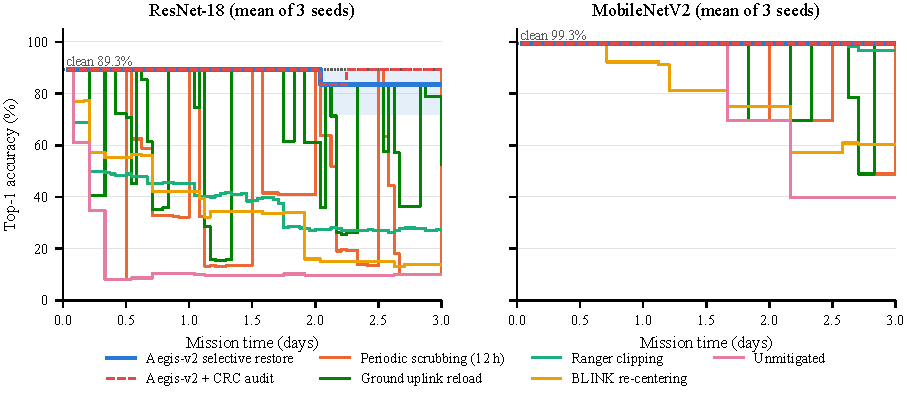
\includegraphics[width=\textwidth]{figures/fig_accuracy.pdf}
\caption{Accuracy over the mission, averaged over three seeds (shaded: min--max across seeds for \aegis{}). Unprotected
ResNet-18 reaches chance ($10\%$) within eight hours. Scrubbing recovers fully at each 12-hour reload and then decays as
new upsets arrive; the ground uplink recovers only during contacts. \aegis{} stays at the clean line except where a
sub-threshold fault in one seed escapes the behavioral gate (day 2); the CRC audit variant repairs it at the next audit.}
\label{fig:accuracy}
\end{figure*}

\subsection{Accuracy Under Accumulating Upsets}
Table~\ref{tab:main} and Fig.~\ref{fig:accuracy} give the main results. On ResNet-18, with $147$ upsets per day and $4.9$
on the exponent MSB, the unprotected model is at chance for almost the entire mission (mean $14.0\%$, final $10.0\%$ in
every seed). Range clipping and BN re-centering slow the collapse but cannot reverse it, because the corrupted weights
stay in memory and accumulate (means $38.5\%$ and $34.0\%$, ending at $27.1\%$ and $13.6\%$). Twelve-hour scrubbing returns
the model to clean accuracy at each reload but spends most of each interval broken (mean $37.0\%$). The ground uplink
repairs only during contacts (mean $66.2\%$). \aegis{} holds $87.4\%$ against a clean $89.3\%$; with the CRC audit,
$88.9\%$, with a final accuracy equal to clean in every seed.

Fig.~\ref{fig:seeds} and Table~\ref{tab:perseed} break the result down by seed. In seeds 0 and 2 all three \aegis{}
variants hold clean accuracy for the entire mission. The gap in the mean comes from a single event: at hour 49 of
seed~1 a sub-threshold weight fault ($0.106\to1.7$) removed 17 points without raising any alarm and persisted to the end
of the mission; the audit variant repaired it at the next six-hourly audit. The baselines vary far more between seeds
(Ranger from $12.7\%$ to $55.3\%$), because a single early exponent hit decides most of their mission.

\begin{figure*}[t]
\centering
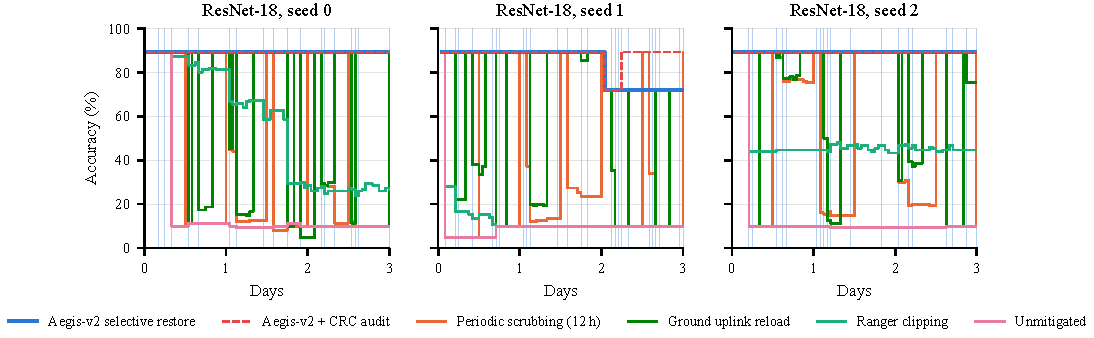
\includegraphics[width=\textwidth]{figures/fig_seeds.pdf}
\caption{Per-seed accuracy for ResNet-18 (faint vertical lines: steps in which \aegis{} restored at least one block).
In seed~1 an undetected sub-threshold fault at hour 49 costs plain \aegis{} 17 points until the end; the audit variant
recovers within six hours.}
\label{fig:seeds}
\end{figure*}

\begin{table}[t]
\centering
\caption{Per-seed mean accuracy in \%, with final accuracy in parentheses.}
\label{tab:perseed}
\setlength{\tabcolsep}{3pt}
\begin{tabular}{@{}lccc@{}}
\toprule
Strategy & Seed 0 & Seed 1 & Seed 2 \\
\midrule
\tablebody{tables/tab_perseed.tex}
\bottomrule
\end{tabular}
\end{table}

Combining Ranger with \aegis{} gives identical accuracy here and $24\%$ less traffic; its restore events are as frequent
(63 versus 62 over all seeds), so the saving comes from restoring fewer or smaller blocks per event, and we have not
isolated the mechanism. MobileNetV2 stores five times fewer bits and is hit five times less often (29 upsets/day). Its
ReLU6 activations are bounded by construction, which plausibly explains why range clipping is far more effective on it
($98.8\%$) than on ResNet-18. All three \aegis{} variants hold the clean $99.3\%$ in every MobileNetV2 seed.

\subsection{Paired Comparison}
Because every strategy sees the same faults within a seed, Table~\ref{tab:paired} reports paired differences. On
ResNet-18 \aegis{} beats every non-\aegis{} baseline in all three seeds: by $+50.5$ points over 12-hour scrubbing, $+21.2$
over the ground uplink, $+48.9$ over range clipping, $+53.4$ over BN re-centering and $+73.4$ over no protection. On
MobileNetV2 the differences are smaller and, except against BN re-centering, not significant with three seeds; in seed~2
no fault was damaging enough to separate any strategies.

\begin{table}[t]
\centering
\caption{Paired difference in mean accuracy, \aegis{} minus baseline (points, 95\% interval), and seeds where \aegis{} was higher.}
\label{tab:paired}
\setlength{\tabcolsep}{3.5pt}
\begin{tabular}{@{}lrcrc@{}}
\toprule
& \multicolumn{2}{c}{ResNet-18} & \multicolumn{2}{c}{MobileNetV2} \\
\cmidrule(lr){2-3}\cmidrule(l){4-5}
Baseline & $\Delta$ & wins & $\Delta$ & wins \\
\midrule
Scrubbing (12 h) & $+50.5\pm23.6$ & 3/3 & $+12.1\pm26.1$ & 2/3 \\
Ground uplink & $+21.2\pm5.3$ & 3/3 & $+6.0\pm12.9$ & 2/3 \\
Ranger clipping & $+48.9\pm48.2$ & 3/3 & $+0.5\pm1.4$ & 2/3 \\
BLINK re-centering & $+53.4\pm36.4$ & 3/3 & $+19.8\pm17.1$ & 3/3 \\
Unmitigated & $+73.4\pm4.8$ & 3/3 & $+22.4\pm51.7$ & 2/3 \\
\aegis{} + audit & $-1.5\pm6.6$ & 0/3 & $0.0\pm0.0$ & 0/3 \\
\bottomrule
\end{tabular}
\end{table}

\subsection{Availability and Accuracy-Loss Area}
Mean accuracy hides how the loss is distributed in time. Table~\ref{tab:availability} reports availability, the share of
the mission spent within five points of clean accuracy, and the accuracy-loss area. On ResNet-18 \aegis{} is available
$89\%$ of the time and the audit variant $98\%$, against $26\%$ for 12-hour scrubbing, $59\%$ for the ground uplink and
under $15\%$ for clipping, re-centering and no protection. The loss areas differ by more than an order of magnitude: 139
point-hours for \aegis{} and 29 with the audit, against 1,663 for the uplink and 3,771 for scrubbing. On MobileNetV2 every
\aegis{} variant is available for the whole mission with zero loss area, while scrubbing and the uplink lose 872 and 432
point-hours.

\begin{table}[t]
\centering
\caption{Availability $\mathcal U$ (\% of mission within 5 points of clean, 95\% interval) and accuracy-loss area $\mathcal L$ (point-hours, mean of seeds).}
\label{tab:availability}
\setlength{\tabcolsep}{3pt}
\begin{tabular}{@{}lrrrr@{}}
\toprule
& \multicolumn{2}{c}{ResNet-18} & \multicolumn{2}{c}{MobileNetV2} \\
\cmidrule(lr){2-3}\cmidrule(l){4-5}
Strategy & $\mathcal U$ (\%) & $\mathcal L$ & $\mathcal U$ (\%) & $\mathcal L$ \\
\midrule
\tablebody{tables/tab_availability.tex}
\bottomrule
\end{tabular}
\end{table}

\subsection{Accuracy per Byte: the Bandwidth Verdict}
\begin{figure*}[t]
\centering
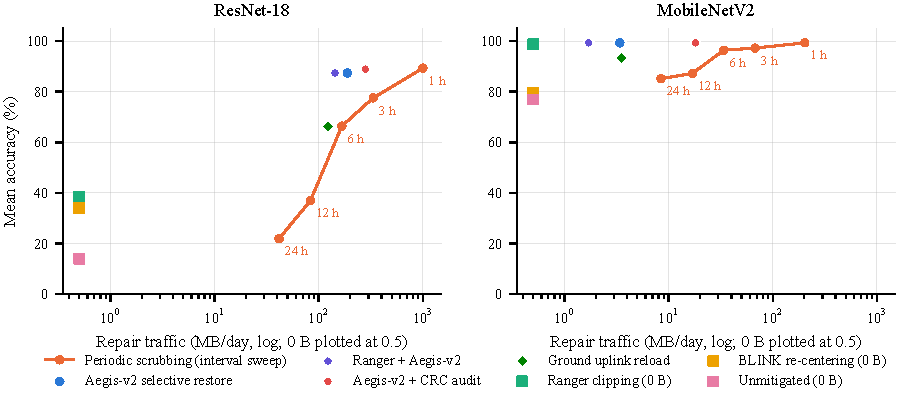
\includegraphics[width=\textwidth]{figures/fig_pareto.pdf}
\caption{Mean accuracy versus repair traffic. The orange curve sweeps the scrubbing interval from 24\,h to 1\,h;
strategies that move no bytes are drawn at $0.5$\,MB/day. All \aegis{} variants lie above and to the left of the
scrubbing frontier on both architectures.}
\label{fig:pareto}
\end{figure*}

Scrubbing has one knob, the interval, which trades traffic for accuracy along the curve of Fig.~\ref{fig:pareto}. No
interval dominates any \aegis{} variant on either architecture. Interpolating the frontier, scrubbing needs about
$889$\,MB/day to reach \aegis{}'s $87.4\%$ on ResNet-18, $4.7\times$ the $188$\,MB/day \aegis{} moves; $975$\,MB/day to match
the audit variant ($3.5\times$); and the combination with Ranger reaches the same accuracy as \aegis{} at $6.2\times$ less
traffic than the matching scrub. On MobileNetV2 the ratio is about $60\times$, mostly because \aegis{} moves almost nothing
($3.4$\,MB/day, nine restore events over all seeds) while the matching 1-hour scrub rewrites the model 24 times a day.

The comparison is at \emph{equal accuracy}. In absolute terms \aegis{} on ResNet-18 moves more bytes than 12-hour
scrubbing (Fig.~\ref{fig:traffic}): it restores on demand, about seven times a day, while the 12-hour scrub moves the
model only twice; but the scrub buys $37\%$ mean accuracy with those bytes and \aegis{} buys $87\%$.

\begin{figure*}[t]
\centering
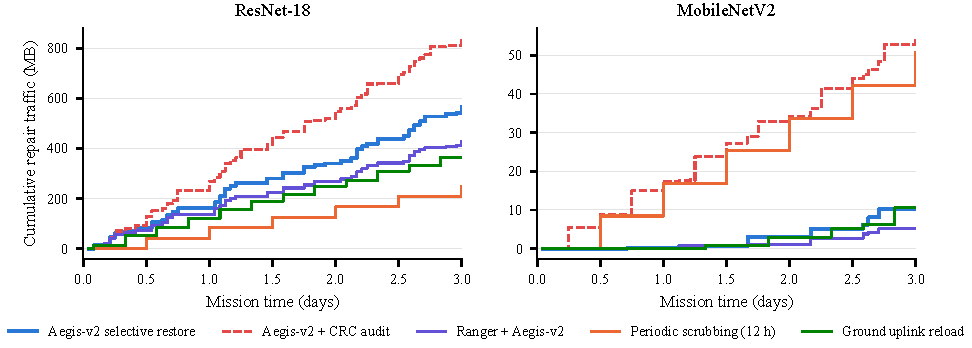
\includegraphics[width=\textwidth]{figures/fig_traffic_time.pdf}
\caption{Cumulative repair traffic (mean of seeds). On ResNet-18 \aegis{} restores on demand and moves more bytes than
12-hour scrubbing, at far higher accuracy (Table~\ref{tab:main}); on MobileNetV2 it moves less than any timer-based scrub.}
\label{fig:traffic}
\end{figure*}

\subsection{Repair Activity and Where Faults Land}
\label{sec:faults}
\begin{figure}[t]
\centering
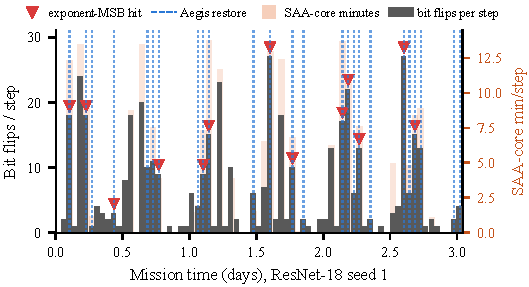
\includegraphics[width=\columnwidth]{figures/fig_faults.pdf}
\caption{Upsets per one-hour step for ResNet-18 seed~1 against SAA-core minutes in the step. Upsets cluster in SAA
passes; exponent-MSB hits (triangles) arrive about five times a day; dashed lines mark steps where \aegis{} restored at
least one block.}
\label{fig:faults}
\end{figure}

Fig.~\ref{fig:faults} shows the arrival process for one seed: upsets bunch into the consecutive daily SAA passes, and
quiet hours alternate with bursts of 20--30 flips. Classifying every recorded hit by the relative change it caused
(destructive: non-finite, exponent MSB, NaN-producing variance sign flip or more than $10^3\times$; moderate: more than
$3\times$; otherwise negligible), only $3.4\%$ of ResNet-18 hits are destructive and $77.9\%$ negligible
(Table~\ref{tab:faults}). Table~\ref{tab:repairs} summarizes repair activity: \aegis{} restores in $29\%$ of ResNet-18 steps,
about seven events a day of $27$\,MB each, and in $4\%$ of MobileNetV2 steps.

\begin{table}[t]
\centering
\caption{Repair activity (mean per seed over three days).}
\label{tab:repairs}
\setlength{\tabcolsep}{3pt}
\begin{tabular}{@{}lrr@{}}
\toprule
 & ResNet-18 & MobileNetV2 \\
\midrule
\tablebody{tables/tab_repairs.tex}
\bottomrule
\end{tabular}
\end{table}

Table~\ref{tab:blocks} explains the traffic: faults land where the bits are, and on ResNet-18 the four
\texttt{layer3}/\texttt{layer4} blocks hold $94\%$ of the parameters, received $95\%$ of the hits and account for $92\%$ of
the 162 block restores. They also show that \aegis{} restores more often than destructive hits occur
(\texttt{layer3.1}: 3 destructive hits, 40 restores): moderate faults that shift batch-norm statistics trigger T2 and are
repaired too, and a block may be restored repeatedly as new hits arrive. Layer selectivity saves the most when damage
is confined to small blocks; for a model whose parameters concentrate at the end, a restore is a large fraction of a
full scrub, and the saving comes mainly from \emph{not} restoring when nothing is wrong.

\begin{table}[t]
\centering
\caption{ResNet-18 blocks: size, share of stored bits, recorded hits, destructive hits and \aegis{} restores (three seeds).}
\label{tab:blocks}
\setlength{\tabcolsep}{3.5pt}
\begin{tabular}{@{}lrrrrr@{}}
\toprule
Block & MB & Bits (\%) & Hits & Destr. & Restores \\
\midrule
\tablebody{tables/tab_blocks.tex}
\bottomrule
\end{tabular}
\end{table}

\subsection{Ablation: the Upstream-Block Rule}
\label{sec:ablation}
Our first GPU campaign ran before the upstream rule existed, with the same seeds and the same injector. Its fault
streams are identical to the final campaign's (same flip counts and exponent hits in every seed), and the baselines
reproduce, so it isolates the rule exactly (Table~\ref{tab:ablation}, Fig.~\ref{fig:ablation}). In seed~1, at hour~17 a
sign flip on \texttt{layer3.0.bn2.running\_var} produced NaN. Its symptoms first appeared at the hooks of the next block,
whose checksum was intact, so nothing was restored and both \aegis{} replicas fell to $10\%$. Plain \aegis{} recovered an
hour later, when an unrelated alarm happened to checksum the culprit; Ranger + \aegis{}, whose clamps changed which
layers alarmed, stayed at chance for 35 hours. With the rule, neither replica dropped. The rule raises Ranger + \aegis{}
from $45.7\%$ to $83.5\%$ mean accuracy in that seed and costs one extra checksum per alarm.

\begin{table}[t]
\centering
\caption{Ablation of the upstream-block rule on identical fault streams (ResNet-18). Mean accuracy (\%) without / with
the rule; last two columns: final accuracy of Ranger + \aegis{}.}
\label{tab:ablation}
\setlength{\tabcolsep}{2.6pt}
\begin{tabular}{@{}lrrrrrrr@{}}
\toprule
& & \multicolumn{2}{c}{\aegis{}} & \multicolumn{2}{c}{+ Ranger} & \multicolumn{2}{c}{final (+R)} \\
\cmidrule(lr){3-4}\cmidrule(lr){5-6}\cmidrule(l){7-8}
Seed & Flips & w/o & with & w/o & with & w/o & with \\
\midrule
\tablebody{tables/tab_ablation.tex}
\bottomrule
\end{tabular}
\end{table}

\begin{figure}[t]
\centering
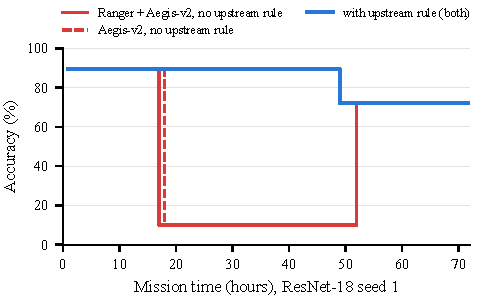
\includegraphics[width=\columnwidth]{figures/fig_ablation.pdf}
\caption{Seed~1 of ResNet-18 with and without the upstream rule, same fault stream. A BN-variance sign flip at hour 17
sends both replicas to chance without the rule; Ranger + \aegis{} stays there for 35 hours.}
\label{fig:ablation}
\end{figure}

\subsection{Single-Fault Detection Study}
\label{sec:detection}
The campaigns show what \aegis{} achieves; they do not show what each tier sees. We therefore injected one persistent
upset at a time into the clean model, 30 trials per bit field and architecture (300 in total), placed like the campaign
injector (block and tensor in proportion to their bits) but with the bit field controlled. Each trial runs one
monitored 16-image batch, records which tiers fired and which blocks T3 confirmed, measures the accuracy loss on the 150
labeled chips, and resets the model (Table~\ref{tab:detection}, Fig.~\ref{fig:detection}).

\begin{table*}[t]
\centering
\caption{Single-fault detection study (30 trials per bit field and architecture). Damaging = loses more than one
evaluation chip. Recall = damaging trials with a T1 or T2 alarm. Localized = alarmed trials in which T3 confirmed the
struck block. False restores = blocks restored that were not struck.}
\label{tab:detection}
\setlength{\tabcolsep}{5pt}
\begin{tabular}{@{}lrrrrrrr@{}}
\toprule
Bit field & Damaging & Loss (pts) & T1 (\%) & T2 (\%) & Recall & Localized (\%) & False restores \\
\midrule
\tablebody{tables/tab_detection.tex}
\bottomrule
\end{tabular}
\end{table*}

\begin{figure*}[t]
\centering
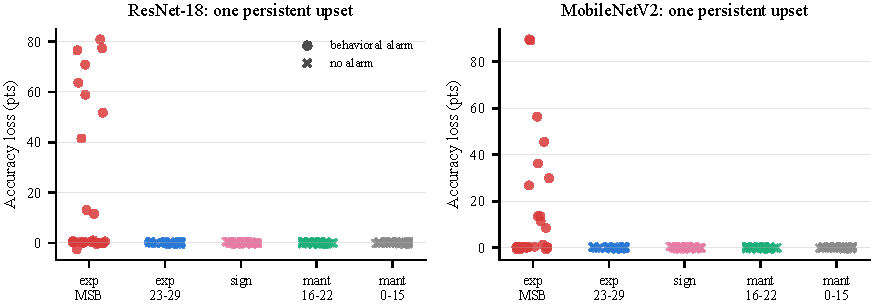
\includegraphics[width=\textwidth]{figures/fig_detection.pdf}
\caption{Accuracy loss of single persistent upsets by bit field (jittered). Circles: a behavioral tier raised an alarm;
crosses: no alarm. Only exponent-MSB flips cause damage, and every damaging flip was detected on both architectures.}
\label{fig:detection}
\end{figure*}

Three findings stand out. \emph{Damage is concentrated in one bit.} Only exponent-MSB flips caused any loss: 12 of 30 on
each architecture, with losses up to 81 points on ResNet-18 and 89 on MobileNetV2. None of the 240 flips in the other
fields lost a single chip, consistent with Table~\ref{tab:bitfields}. Weighting by field size, about $1.3\%$ of uniformly
placed flips are damaging ($\tfrac{1}{32}\times40\%$), the same order as the $3\%$ failure rate reported for FP32 flips
in vision transformers~\cite{sentry2026}. \emph{Every damaging flip was detected and localized.} Recall was 12/12 on both
models, T3 confirmed the struck block in every alarmed exponent-MSB trial, and no trial restored a block that had not been
struck. The 18 non-damaging exponent-MSB flips per model also raised alarms and were restored; they are real corruptions
that happened not to cost accuracy on these chips, and restoring them prevents latent damage. \emph{Behavioral tiers are
noisy, the checksum is not.} On ResNet-18, $12.5\%$ of the 120 harmless trials raised a T1 alarm, always at
\texttt{layer4.0}, independent of where the fault was: some clean batches exceed the calibrated envelope of that layer.
T3 checked \texttt{layer4.0} and its upstream block, found both intact, and restored nothing (in the two sign-flip trials
where the struck block happened to be one of those two, it was correctly restored). MobileNetV2 raised no such alarms.
The CRC gate is therefore what keeps an imperfect behavioral monitor cheap: its false alarms cost a checksum of two
blocks ($\approx3$\,mJ on ResNet-18), never a restore, which also explains the large T3 share of ResNet-18's energy
(Table~\ref{tab:energy}).

The study does not contradict the sub-threshold miss in the campaign (Fig.~\ref{fig:seeds}). That fault
($0.106\to1.7$, a factor of 16) came from an exponent bit below the MSB and kept every activation inside its envelope.
None of our 30 sub-MSB exponent trials reproduced such a loss on a clean model: a sixteen-fold change to a weight that
matters is rare under uniform placement, and in the campaign it arrived on a model that had already absorbed dozens of
upsets. Rare, behaviorally silent faults of this kind are exactly what the periodic audit is for.

\subsection{What a Damaged Classifier Predicts}
\label{sec:collapse}
For an Earth-observation product the failure mode matters as much as the failure rate. Fig.~\ref{fig:confusion} pools
the confusion matrices of the eight ResNet-18 trials that lost more than 20 points. Damage does not produce structured
semantic confusions such as River$\leftrightarrow$Highway; it collapses the classifier toward one class that depends on the
fault. In those trials a single class absorbed $56$--$82\%$ of all predictions (Highway in three trials, River in two,
Annual Crop, Herbaceous Vegetation and Pasture in one each); two MobileNetV2 trials collapsed completely, labelling all
150 chips as Sea/Lake and as Highway respectively. A downstream consumer would see a confident, plausible-looking
stream of one land-cover class, which is why silent corruption must be detected onboard rather than inferred from the
product.

\begin{figure*}[t]
\centering
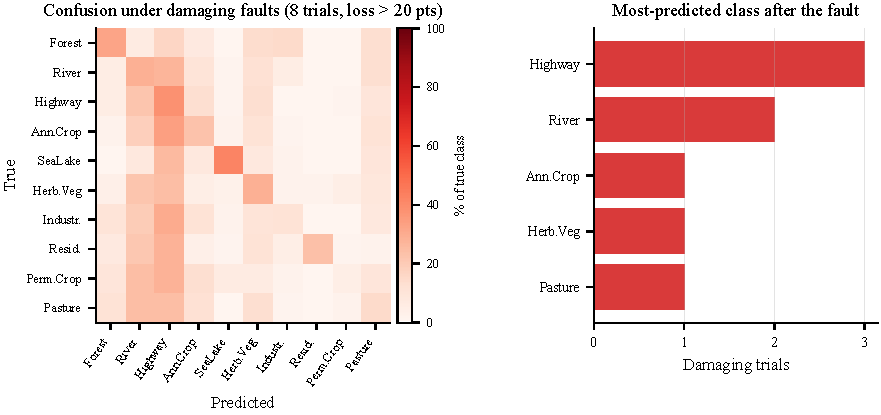
\includegraphics[width=\textwidth]{figures/fig_confusion.pdf}
\caption{Left: pooled row-normalized confusion matrix of ResNet-18 under the eight single upsets that cost more than 20
points. Right: the class that received the most predictions in each of those trials. A damaging upset collapses the
classifier toward a fault-dependent class rather than producing semantically structured confusions.}
\label{fig:confusion}
\end{figure*}


\subsection{Transient Faults Do Not Trigger Restores}
\label{sec:transient}
A behavioral monitor alone cannot distinguish a transient glitch in an activation buffer from corrupted weights. We
injected exponent-MSB flips into activations, not weights, in 40 single-batch trials on ResNet-18
(Table~\ref{tab:transient}). Tier 1 or 2 raised an alarm in $27.5\%$ of trials; Tier 3 found no checksum mismatch in any,
so no bytes were moved. This is the second purpose of the CRC gate: beyond localizing cascades, it makes repair
decisions robust to faults that need no repair.

\begin{table}[t]
\centering
\caption{Transient activation faults (ResNet-18).}
\label{tab:transient}
\setlength{\tabcolsep}{3pt}
\begin{tabular}{@{}lr@{}}
\toprule
\tablebody{tables/tab_transient.tex}
\bottomrule
\end{tabular}
\end{table}

\subsection{Energy: a Negative Result}
\label{sec:costs}
\begin{figure}[t]
\centering
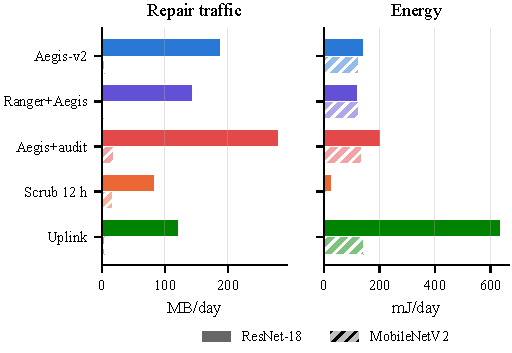
\includegraphics[width=\columnwidth]{figures/fig_costs.pdf}
\caption{Repair traffic and modeled energy per day. Solid: ResNet-18; hatched: MobileNetV2.}
\label{fig:costs}
\end{figure}

\begin{figure}[t]
\centering
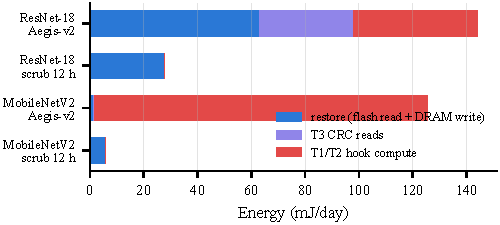
\includegraphics[width=\columnwidth]{figures/fig_energy_breakdown.pdf}
\caption{Where \aegis{}'s energy goes, against 12-hour scrubbing.}
\label{fig:energy}
\end{figure}

Fig.~\ref{fig:costs} separates the two costs. Under our energy model \aegis{} spends $144$\,mJ/day on ResNet-18 and
$126$\,mJ/day on MobileNetV2, versus $27.9$ and $5.7$\,mJ/day for 12-hour scrubbing: $5.2\times$ and $22\times$ more.
Fig.~\ref{fig:energy} and Table~\ref{tab:energy} show why. On ResNet-18, restores are $44\%$ of the energy, T3 checksum
reads $24\%$ and the T1/T2 hooks $32\%$; on MobileNetV2 the hooks are $99\%$, because restores are rare and its expanded
activations make elementwise monitoring expensive (Table~\ref{tab:complexity}). Our first prototype claimed a $98.9\%$
energy saving because it did not charge the monitor; that claim was wrong. With the monitor charged, \aegis{} is an
energy \emph{cost}, and our claim is about bandwidth and availability.

\begin{table}[t]
\centering
\caption{\aegis{} energy by component (mJ/day, share of total).}
\label{tab:energy}
\setlength{\tabcolsep}{2.5pt}
\begin{tabular}{@{}lrrrr@{}}
\toprule
 & Restore & T3 CRC & T1/T2 hooks & Total \\
\midrule
\tablebody{tables/tab_energy.tex}
\bottomrule
\end{tabular}
\end{table}

The result needs perspective. The satellite spends energy on inference anyway: 16 images per hour at the $12.5$\,mJ
ResNet-18 proxy is $4.8$\,J/day, so \aegis{}'s $144$\,mJ/day is $3\%$ of the inference budget and 12-hour scrubbing's
$28$\,mJ/day is $0.6\%$. Two further caveats cut in \aegis{}'s favor: $6.9$\,pJ per elementwise operation is likely
pessimistic for fused hardware reductions, and monitoring could run on every $n$-th batch, trading detection latency
for energy linearly. The ground uplink is the most expensive option by far ($635$\,mJ/day on ResNet-18) because radio
reception costs more than an order of magnitude more per bit than memory.

\subsection{Cross-Architecture Observations}
The two architectures agree on the ordering of the \aegis{} variants and on the failure of blind timers, and disagree
on the baselines. MobileNetV2 is hit five times less often, so its unprotected mean ($76.9\%$) is far above ResNet-18's,
and range clipping nearly matches \aegis{} on it. The monitoring cost moves the other way: elementwise hooks are $16\%$ of
MobileNetV2's inference arithmetic against $1\%$ for ResNet-18. A compact model with bounded activations therefore
shifts the balance toward cheap in-place mitigation, while a large model with unbounded activations makes detection-gated
repair indispensable.

% =====================================================================================================
\section{Lessons: Pitfalls That Invalidated Results}
\label{sec:lessons}
Table~\ref{tab:pitfalls} lists the mistakes that each silently produced a plausible but wrong result during this work,
with the invariant that now prevents them. We list them because each is easy to repeat elsewhere; the fixes are covered
by regression tests in the repository.

\begin{table*}[t]
\centering
\caption{Evaluation pitfalls encountered during this work.}
\label{tab:pitfalls}
\setlength{\tabcolsep}{4pt}
\begin{tabular}{@{}>{\raggedright\arraybackslash}p{2.4cm}>{\raggedright\arraybackslash}p{5.1cm}>{\raggedright\arraybackslash}p{4.5cm}>{\raggedright\arraybackslash}p{4.6cm}@{}}
\toprule
Pitfall & Symptom & Cause & Invariant \\
\midrule
Synthetic inputs & ``98.9\% energy saving'' headline & evaluation on Gaussian-noise tensors, always-on gate, uncharged monitor & never evaluate on random tensors; real EuroSAT chips only \\
Input contract & $\approx18\%$ clean accuracy; chance with wrong labels & 64\,px input; alphabetical label order & 224\,px bicubic, dataset statistics, checkpoint label order \\
Envelope statistics & restores on every step & mean$\pm k\sigma$ bounds on heavy-tailed activations & observed extrema + margin over $\ge100$ chips \\
Calibration leakage & optimistic detection & calibration and evaluation chips overlap & disjoint splits; trained models exclude both \\
Poisoned reference & fault becomes undetectable & golden CRCs refreshed while corrupt & re-baseline only blocks just restored \\
Hook placement & 35 h at chance (Table~\ref{tab:ablation}) & BN fault seen one block downstream & always checksum the upstream block \\
Name mapping & every MobileNetV2 alarm sent to stem & two diverging layer-to-block mappings & one mapping function for keys and modules \\
Fault field & inflated severity & exponent-only injection ($4\times$ MSB rate) & uniform over all 32 bits; disclose any restriction \\
Uncharged costs & energy cost reported as saving & monitor, CRC or recalibration not charged & charge hooks, CRC reads, recalibration inferences \\
\bottomrule
\end{tabular}
\end{table*}

% =====================================================================================================
\section{Discussion}
\label{sec:discussion}

\textbf{Why gating works.} Most upsets are harmless: $72.5\%$ hit mantissas and $77.9\%$ change a weight by less than a
factor of three. A blind scrubber pays for all of them; an in-place mitigator pays for none of them but cannot undo the
rare catastrophic one. \aegis{} pays only when behavior \emph{and} checksums agree that something is broken, which is what
lets it sit above the scrubbing frontier.

\textbf{When it does not.} The behavioral gate has a blind spot, faults large enough to matter but too small to move
activations past calibrated bounds (Section~\ref{sec:detection}). The audit closes it at a cost that scales with model
size and audit frequency; a mission could schedule audits after SAA exits, when new faults are most likely, instead of
on a fixed clock. Gating also cannot help when monitoring itself dominates energy (MobileNetV2), and it cannot repair
the golden copy, whose integrity rests on rad-tolerant storage and its own ECC.

\textbf{Choosing a strategy.} Table~\ref{tab:guide} distills the results into guidance. If uplink and memory traffic are
the scarce resources and availability matters, detection-gated repair with an audit is the best of the evaluated
options. If energy is the binding constraint and long downtime is tolerable, a slow scrub is cheaper. If the
model is small with bounded activations and no golden store is available, range clipping already recovers most of the
accuracy.

\begin{table}[t]
\centering
\caption{Which strategy for which constraint (from the evaluated campaigns).}
\label{tab:guide}
\setlength{\tabcolsep}{3pt}
\begin{tabular}{@{}>{\raggedright\arraybackslash}p{3.2cm}>{\raggedright\arraybackslash}p{4.9cm}@{}}
\toprule
Binding constraint & Best evaluated option \\
\midrule
Availability, bandwidth & \aegis{} + CRC audit (98\% / 100\% available) \\
Bandwidth, low energy & Ranger + \aegis{} (lowest traffic at top accuracy) \\
Energy only & slow scrub (12--24 h); accepts long downtime \\
No golden store, compact model & range clipping (98.8\% on MobileNetV2) \\
No onboard repair possible & ground uplink (only during contacts) \\
\bottomrule
\end{tabular}
\end{table}

\textbf{Deployment.} The golden copy fits comfortably in MRAM or rad-hard NOR for models of this size, or in $9.2$\,MB with
INT8 at a small accuracy cost. T3 needs only a CRC engine and a table of 32-bit references; T1/T2 need reductions over
activations that many accelerators can fuse into the layers that produce them. The method is complementary to ECC: with
ECC on the working memory, \aegis{} would act on the residue of uncorrectable and logic-induced errors that beam studies
show ECC misses~\cite{dossantos2023neutron}.

% =====================================================================================================
\section{Threats to Validity}
\label{sec:validity}
\textbf{Radiation model.} Rates are transferred from Alsat-1 (686\,km, 2002-era SRAM) to Sentinel-2A at 786\,km and to
modern memory, whose sensitivity can differ by orders of magnitude. The SAA-to-background ratio is assumed, the IGRF
ramp is a proxy for a trapped-proton flux model such as AP8/AE9 combined with device cross-sections, solar-cycle
variation is not modeled, and faults are injected only into parameters, not into control logic or activation buffers,
which beam studies show can dominate~\cite{dossantos2023neutron}.
\textbf{Statistics.} Three seeds and 150 evaluation chips give wide intervals; one chip is $0.67$ points. The MobileNetV2
paired differences are mostly not significant.
\textbf{Energy.} All energy constants are analytic proxies, not measurements on flight hardware, and Ranger/BLINK compute
is not charged, which flatters those baselines.
\textbf{Models.} The ResNet-18 checkpoint's training split is unknown; MobileNetV2 has a verified held-out split.
\textbf{Mission length.} Three days captures several SAA cycles and dozens of exponent-MSB hits, but not long-term effects
such as total ionizing dose.
\textbf{Ablation.} The pre-fix campaign predates other small code changes; its fault streams and baselines match the
final campaign, but its numbers outside the ablated strategies should not be cited.
\textbf{Literature.} Several closely related works are 2026 preprints; we checked their records but cite their results as
reported.

% =====================================================================================================
\section{Future Work}
Natural extensions are (i)~orbit-aware scheduling of audits and monitoring duty cycle around SAA passes, which targets
both the blind spot and the energy cost; (ii)~a physics-based environment (AP8/AE9 with device cross-sections via SPENVIS
or CREME96); (iii)~measured energy and latency on a Jetson- or NPU-class board; (iv)~activation and logic faults alongside
weight faults, with neutron-beam validation; (v)~vision transformers and larger EO tasks such as segmentation; and
(vi)~longer missions spanning a solar-cycle phase.

% =====================================================================================================
\section{Conclusion}
Onboard classifiers in LEO accumulate silent, sometimes catastrophic weight corruption. We showed that combining cheap
behavioral signals with exact checksums lets a satellite repair only what is broken, when it is broken: on an
orbit-calibrated, paired simulation of a Sentinel-2A mission, \aegis{} kept a ResNet-18 within two points of clean
accuracy and available $89\%$ of the time ($98\%$ with the audit), where 12-hour scrubbing, range clipping, re-centering
and ground reload lost 23 to 55 points, and it did so with several times less repair traffic than the scrubbing interval
that would match it. An exact ablation showed that one small rule, checksumming the block upstream of an alarm, prevents
day-long outages. The same analysis showed what the method does not do: with honest accounting, always-on monitoring
costs more energy than a slow scrub. We hope the simulator, the pitfalls and the results help the next design start
from realistic faults and complete budgets.

\section*{Acknowledgment}
The author thanks the maintainers of EuroSAT, PyTorch, sgp4, ppigrf and CelesTrak, whose open data and software made this
study possible.

\appendices
\section{Reproducibility}
All results come from \texttt{results/main\_final}, \texttt{results/main\_final\_mobilenet},
\texttt{results/main\_gpu} (ablation), \texttt{results/transient\_faults.json} and \texttt{results/detection\_study\_*.json}.
To regenerate:
\begin{scriptsize}
\begin{verbatim}
python experiments/run_campaign.py --days 3 \
  --seeds 0 1 2 --eval-per-class 15 \
  --scrub-sweep-hours 1 3 6 24 --name main_final
python experiments/train_mobilenet.py --epochs 3
python experiments/run_campaign.py ... \
  --arch mobilenet_v2 --name main_final_mobilenet
python experiments/transient_faults.py --trials 40
python experiments/detection_study.py --arch resnet18
python experiments/detection_study.py --arch mobilenet_v2
python researchpaper/make_paper_figures.py
python researchpaper/make_paper_tables.py
\end{verbatim}
\end{scriptsize}
Every seed file records the fault field, orbit model, golden-store format and recalibration flag with its numbers.

\section{Notation}
\begin{center}
\setlength{\tabcolsep}{3pt}
\begin{tabular}{@{}ll@{}}
\toprule
$\theta$, $N$, $B$ & stored model state, values, bits \\
$b_k$, $K$ & block $k$ in forward order, number of blocks \\
$\lambda(t)$, $\lambda_{\mathrm{bg}}$, $\lambda_{\mathrm{SAA}}$ & upset rate; background; SAA core \\
$B_{\mathrm e}$, $B_{\mathrm c}$ & field strength at SAA edge and core \\
$[\ell_l,u_l]$, $\alpha$ & T1 envelope of layer $l$, margin \\
$d_l$, $\tau_l$ & T2 drift score and threshold of BN layer $l$ \\
$g_k$, $\mathcal G$ & golden CRC of block $k$, golden store \\
$A_\pi(t)$, $A_0$ & accuracy of $\pi$ at step $t$; clean accuracy \\
$\bar A_\pi$, $\mathcal U_\pi$, $\mathcal L_\pi$ & mean accuracy, availability, loss area \\
$D_\pi$, $E_\pi$ & bytes moved, energy spent \\
\bottomrule
\end{tabular}
\end{center}

\bibliographystyle{IEEEtran}
\bibliography{references}

\end{document}
